\def\year{2018}\relax
%File: formatting-instruction.tex
\documentclass[letterpaper]{article} %DO NOT CHANGE THIS
\usepackage{aaai18}  %Required
\usepackage{times}  %Required
\usepackage{helvet}  %Required
\usepackage{courier}  %Required
\usepackage{url}  %Required
\usepackage{graphicx}  %Required
\usepackage{subfig}
\usepackage{amsmath}
\usepackage{amsfonts}
\usepackage{amssymb}
\usepackage{amsthm}
\usepackage{bbm}
%\usepackage{color}
%\usepackage{subfiles}
\newtheorem{theorem}{Theorem}
\newtheorem{lemma}{Lemma}
\newtheorem*{corollary*}{Proof Sketch}
\newtheorem{assumption}{Assumption}
\newtheorem{definition}{Definition}
\newtheorem{proposition}{Proposition}
%\usepackage{algorithm}
%\usepackage{algorithmic}
%\newcommand{\theHalgorithm}{\arabic{algorithm}}
%\newcommand{\textit{diag}}{\rm{diag}}
\usepackage[linesnumbered, algoruled]{algorithm2e}

%\renewcommand{\algorithmicrequire}{\textbf{Input:}}
%\renewcommand{\algorithmicensure}{\textbf{Output:}}
\frenchspacing  %Required
\setlength{\pdfpagewidth}{8.5in}  %Required
\setlength{\pdfpageheight}{11in}  %Required
\setlength\titlebox{2.5in}
%PDF Info Is Required:
\pdfinfo{
/Title (Stochastic Non-convex Ordinal Embedding with Stabilized Barzilai-Borwein Step Size)
/Author (Ke Ma, Jinshan Zeng, Jiechao Xiong, Qianqian Xu, Xiaochun Cao, Wei Liu, Yuan Yao)}
\setcounter{secnumdepth}{0}
 \begin{document}
% The file aaai.sty is the style file for AAAI Press
% proceedings, working notes, and technical reports.
%
\title{Stochastic Non-convex Ordinal Embedding with \\Stabilized Barzilai-Borwein Step Size}
%\author
%{
%	Ke Ma, Jinshan Zeng, Jiechao Xiong, Qianqian Xu, Xiaochun Cao, Wei Liu, Yuan Yao\\
%	State Key Laboratory of Information Security, Institute of Information Engineering, Chinese Academy of Sciences\\
%	%No.89(A) Minzhuang Road, Building 3, Haidian District,	Beijing, P.R.China 100093\\
%	School of Cyber Security, University of Chinese Academy of Sciences\\
%	%No.19(A) Yuquan Road, Shijingshan District, \\
%	%Beijing, P.R.China 100049\\
%	School of Computer Information Engineering, Jiangxi Normal University,\\
%	%No.99 Ziyang Avenue\\
%	%Nanchang, Jiangxi, P.R.China 330022\\
%	Department of Mathematics, Hong Kong University of Science and Technology\\
%	%Clear Water Bay, Kowloon, Hong Kong, P.R.China
%	Tencent AI Lab
%}
\author
{
		Ke Ma\textsuperscript{1,2}, Jinshan Zeng\textsuperscript{3,4}, Jiechao Xiong\textsuperscript{5}, Qianqian Xu\textsuperscript{1}, 
		\bf\Large{Xiaochun Cao\textsuperscript{1*}, Wei Liu\textsuperscript{5}, Yuan Yao\textsuperscript{4}\thanks{The corresponding authors.}}\\
		\textsuperscript{1} State Key Laboratory of Information Security, Institute of Information Engineering, Chinese Academy of Sciences\\
		\textsuperscript{2} School of Cyber Security, University of Chinese Academy of Sciences\\
		\textsuperscript{3} School of Computer Information Engineering, Jiangxi Normal University\\
		\textsuperscript{4} Department of Mathematics, Hong Kong University of Science and Technology \textsuperscript{5} Tencent AI Lab\\
		\{make, xuqianqian, caoxiaochun\}@iie.ac.cn, jsh.zeng@gmail.com\\
		jcxiong@tencent.com, wliu@ee.columbia.edu, yuany@ust.hk
}
\maketitle
\begin{abstract}
	Learning representation from relative similarity comparisons, often called ordinal embedding, gains rising attention in recent years. Most of the existing methods are batch methods designed mainly based on the convex optimization, say, the projected gradient descent method. However, they are generally time-consuming due to that the singular value decomposition (SVD) is commonly adopted during the update, especially when the data size is very large. To overcome this challenge, we propose a stochastic algorithm called SVRG-SBB, which has the following features: (a) SVD-free via dropping convexity, with good scalability by the use of stochastic algorithm, i.e., stochastic variance reduced gradient (SVRG), and (b) adaptive step size choice via introducing a new stabilized Barzilai-Borwein (SBB) method as the original version for convex problems might fail for the considered stochastic \textit{non-convex} optimization problem. Moreover, we show that the proposed algorithm converges to a stationary point at a rate $\mathcal{O}(\frac{1}{T})$ in our setting, where $T$ is the number of total iterations. Numerous simulations and real-world data experiments are conducted to show the effectiveness of the proposed algorithm via comparing with the state-of-the-art methods, particularly, much lower computational cost with good prediction performance.
\end{abstract}

\section{Introduction}

 Ordinal embedding aims to learn representation of data objects as points in a low-dimensional space. The distances among these points agree with a set of relative similarity comparisons as well as possible. Relative comparisons are often collected by workers who are asked to answer the following question:
	
\emph{``Is the similarity between object $i$ and $j$ larger than the similarity between $l$ and $k$?"}
	
The feedback of individuals provide us a set of quadruplets, \textit{i.e.}, $\{(i,j,l,k)\}$, which can be treated as the supervision for ordinal embedding. Without prior knowledge, the relative similarity comparisons always involve all objects and the number of potential quadruplet could be $\mathcal{O}(n^4)$.
	
The ordinal embedding problem was firstly studied by \cite{Shepard1962a,Shepard1962b,Kruskal1964a,Kruskal1964b} in the psychometric society. In recent years, it has drawn a lot of attention in machine learning \cite{jamieson2011low,53e99af7b7602d97023851bf,2015arXiv150102861A,NIPS2016_6554}, statistic ranking \cite{McFee:2011:LMS:1953048.1953063,kevin2011active}, artificial intelligence \cite{Heikinheimo2013TheCA,503}, information retrieval \cite{7410580}, and computer vision \cite{wah2014similarity,wilberKKB2015concept}, etc.

One of the typical methods for ordinal embedding problem is the well-known
Generalized Non-Metric Multidimensional Scaling (GNMDS) \cite{agarwal2007generalized}, which aims at finding a low-rank Gram (or kernel) matrix $\mathbf{G}$ in Euclidean space such that the pairwise distances between the embedding of objects in Reproducing Kernel Hilbert Space (RKHS) satisfy the relative similarity comparisons. As GNMDS uses hinge loss to model the relative similarity between the objects, it neglects the information provided by satisfied constraints in finding the underlying structure in the low-dimensional space. To alleviate this issue, the Crowd Kernel Learning (CKL) was proposed by \cite{tamuz2011adaptiive} via employing a scale-invariant loss function. However,
the objective function used in CKL
%CKL suffers from the problem that this objective function
only considers the constraints which are strongly violated.
%On the other hand,
Latter, \cite{vandermaaten2012stochastic} proposed the Stochastic Triplet Embedding (STE) that jointly penalizes the violated constraints and rewards the satisfied constraints, via using the logistic loss function. Note that the aforementioned three typical methods are based on the convex formulations, and also employ the projected gradient descent method and singular value decomposition (SVD) to obtain the embedding.
However, a huge amount of comparisons and the computational complexity of SVD significantly inhibit their usage to large scale and on-line applications. Structure Preserving Embedding (SPE) \cite{Shaw:2009:SPE:1553374.1553494} and Local Ordinal Embedding (LOE) \cite{Terada2014LocalOE} embed unweighted nearest neighbor graphs to Euclidean spaces with convex and non-convex objective functions. The nearest neighbor adjacency matrix can be transformed into ordinal constraints, but it is not a standard equipment in those scenarios which involve relative comparisons. With this limitation, SPE and LOE are not suitable for ordinal embedding via quadruplets or triple comparisons.
	
In contrast to the kernel-learning or convex formulation of ordinal embedding, the aforementioned methods have the analogous non-convex counterparts. The non-convex formulations directly obtain the embedding instead of the Gram matrix. Batch gradient descent is not suitable for solving these large scale ordinal embedding problems because of the expense of full gradients in each iteration. Stochastic gradient descent (SGD) is a common technology in this situation as it takes advantage of the stochastic gradient to devise fast computation per iteration.
In \cite{ghadimi2013stochastic}, the $\mathcal{O}(\frac{1}{\sqrt{T}})$ convergence rate of SGD for the stochastic non-convex optimization problem was established, in the sense of convergence to a stationary point, where $T$ is the total number of iterations.
%A non-asymptotic convergence analysis of SGD for stochastic non-convex optimization problem is established which attains a convergence rate of ().
As SGD has slow convergence due to the inherent variance, stochastic variance reduced gradient (SVRG) method was proposed in \cite{rie2013accelerating} to accelerate SGD.
For the strongly convex function, the linear convergence of SVRG with Option-II was established in \cite{rie2013accelerating}, and latter the linear convergence rates of SVRG with Option-I and SVRG incorporating with the Barzilai-Borwein (BB) step size were shown in \cite{NIPS2016_6286}.
In the non-convex case, the $\mathcal{O}(\frac{1}{T})$ convergence rates of SVRG in the sense of convergence to a stationary point were shown in \cite{pmlr-v48-reddi16,pmlr-v48-allen-zhua16} under certain conditions.
% for strongly and smooth convex functions.
%The convergence rate of non-convex finite-sum problems can be improved via SVRG \cite{pmlr-v48-reddi16,pmlr-v48-allen-zhua16} as .


%One of the major issues in stochastic optimization is choosing an appropriate step size.
Although the BB step size has been incorporated into SVRG and its effectiveness has been shown in
 \cite{NIPS2016_6286} for the strongly convex case, it might not work when applied to some stochastic non-convex optimization problems.
 %, especially, the stochastic non-convex ordinal embedding studied in this paper.
Actually, in our latter simulations, we found that the absolute value of the original BB step size is unstable when applied to the stochastic non-convex ordinal embedding problem studied in this paper (see, Figure \ref{fig:step}(a)). The absolute value of the original BB step size varies dramatically with respect to the epoch number.
 %However, the BB technique incorporated in \cite{NIPS2016_6286} can not be directly applied to the \textit{non-convex} problem,
Such phenomenon is mainly due to without the strong convexity, the denominator of BB step size might be very close 0, and thus the BB step size broken up. This motivates us to investigate some new stable and adaptive strategies of step size for SVRG when applied to the stochastic non-convex ordinal embedding problem.


In this paper, we introduce a new adaptive step size strategy called stabilized BB (SBB) step size via adding another positive term to the absolute of the denominator of the original BB step size to overcome the instability of the BB step size, and then propose a new stochastic algorithm called SVRG-SBB via incorporating the SBB step size for fast solving the considered non-convex ordinal embedding model. In a summary, our main contribution can be shown as follows:	
\begin{itemize}
\item
We propose a non-convex framework for the ordinal embedding problem via considering the optimization problem with respect to the original embedding variable but not its Gram matrix. By exploiting this idea, we get rid of the positive semi-definite (PSD) constraint on the Gram matrix, and thus, our proposed algorithm is SVD-free and has good scalability. %To the best of our knowledge, it is the first work to study the ordinal embedding problem in such non-convex framework.

\item
The introduced SBB step size can overcome the instability of the original BB step size when the original BB step size does not work. More importantly, the proposed SVRG-SBB algorithm outperforms most of the the state-of-the-art methods as shown by numerous simulations and real-world data experiments, in the sense that SVRG-SBB often has better generalization performance and significantly reduces the computational cost.

\item We establish $O(\frac{1}{T})$ convergence rate of SVRG-SBB in the sense of convergence to a stationary point, where $T$ is the total number of iterations. Such convergence result is comparable with the existing best convergence results in literature.
\end{itemize}

%{\bf Organization:}
%The rest of this paper is organized as follows. Section 2 describes the stochastic ordinal embedding problem. Section 3 shows the development of the proposed algorithm as well as the establishment of its convergence rate. Section 4 provides a series of simulations and real-world data experiments to demonstrate the effectiveness of the proposed algorithm. We conclude this paper in Section 5.

%Congratulations on having a paper selected for inclusion in an AAAI Press proceedings or technical report! This document details the requirements necessary to get your accepted paper published using \LaTeX{}. If you are using Microsoft Word, instructions are provided in a different document. If you want to use some other formatting software, you must obtain permission from AAAI Press first.

%The instructions herein are provided as a general guide for experienced \LaTeX{} users. If you do not know how to use \LaTeX{}, do not use it to format your paper. AAAI cannot provide you with support and the accompanying style files are \textbf{not} guaranteed to work. If the results you obtain are not in accordance with the specifications you received, you must correct your source file to achieve the correct result.

%These instructions are generic. Consequently, they do not include specific dates, page charges, and so forth. Please consult your specific written conference instructions for details regarding your submission. Please review the entire document for specific instructions that might apply to your particular situation. All authors must comply with the following:

%\begin{itemize}
%	\item You must use the 2018 AAAI Press \LaTeX{} style file and bib file, which are located in the 2018 author kit.
%	\item You must complete, sign, and return by the deadline the AAAI copyright form (proceedings authors) or distribution license (technical report authors).
%	\item You must read and format your paper source and PDF according to the formatting instructions for authors.
%	\item You must submit your electronic files and abstract using our electronic submission form \textbf{on time.}
%	\item You must pay any required page or formatting charges to AAAI Press so that they are received by the deadline.
%	\item You must check your paper before submitting it, ensuring that it compiles without error, and complies with the guidelines found in the author kit.
%\end{itemize}

%\section{Related Work}
%	
%\subsection{Ordinal Embedding}
%	
% We briefly review some existed techniques for learning data embedding based on relative similarity comparisons. Generalized Non-Metric Multidimensional Scaling (GNMDS) \cite{agarwal2007generalized} aims to find a low-rank Gram (or kernel) matrix $\mathbf{G}$ in Euclidean space such that the pairwise Euclidean distances between the embedding of the objects in the Reproducing Kernel Hilbert Space (RKHS) satisfy the relative similarity comparisons. As the GNMDS uses the hinge loss to model the relative similarity between the objects, it neglects the information provided by satisfied constraints in finding the underlying structure in the low-dimensional space. Crowd Kernel Learning (CKL) \cite{tamuz2011adaptiive} employs a scale-invariant loss function and alleviates this issue. However, it suffers from the problem that the objective function only considers the constraints which are strongly violated. On the other hand, Stochastic Triplet Embedding (STE) \cite{vandermaaten2012stochastic} adopts a logistic loss function for the same purpose, which jointly penalizes the violated constraints and rewards the satisfied constraints.
%	
%All these methods has the scalability issue significantly inhibiting their usage in applications. In contrast to the kernel-learning or convex formulations, the aforementioned methods have the analogous embedding learning counterparts, i.e. they are non-convex optimization problems, and employ the gradient descent to optimize. The non-convex formulations with gradient descent optimization are not suitable for solving the large scale ordinal embedding problems because of the expense of full gradients in each iteration.
%	
%Structure Preserving Embedding (SPE) \cite{Shaw:2009:SPE:1553374.1553494} and Local Ordinal Embedding (LOE) \cite{Terada2014LocalOE} embed unweighted nearest neighbor graphs to Euclidean spaces with convex and non-convex objective function. The nearest neighbor adjacency matrix can be transformed into ordinal constraints \cite{Terada2014LocalOE}. But the nearest neighbor adjacency matrix is not a standard equipment in those scenarios which involve relative comparisons. With this limitation, SPE and LOE are not suitable for ordinal embedding with quadruplets or triple comparisons.
	
%\subsection{Metric Embedding}
%	
% There exists a huge body of work on algorithms that embed data points based on metric information, such as distance, similarity, co-occurrence, and so on. The metric embedding An overview over the traditional approach of metric multidimensional scaling can be found in \cite{BorgGroenen2005}. The most of the existed  algorithms follow the paradigm that it is enough to preserve local distances: Isomap \cite{Tenenbaum2319}, Locally Linear Embeddings (LLE) \cite{Roweis2323}, Laplacian Eigenmaps \cite{Belkin:2003:LED:795523.795528}, Stochastic Neighbor Embedding (SNE) \cite{NIPS2002_2276}, t-SNE \cite{maaten2008visualizing}, and so on. The main difference between the metric embedding and ordinal embedding is: metric algorithms seek an embedding with inter-point distances closely matching the metric information which is the necessary input; and ordinal algorithms find an embedding respecting only the relative ordering of the metric information instead of the metric information itself. As the magnitude of the metric information is unreliable, too difficult to measure, or simply unavailable, the metric embedding is not appropriate in many of applications associated with human cognition. Althrough the numerical value of metric information that the users give are typically not reliable, the relative ordering of them will be fairly consistent \cite{kendall1948rank}. Ordianl methods are more appropriate in the tasks than metric methods.
	
%\subsection{Non-convex Semi-definite Optimization}
%	
% As GNMDS \cite{agarwal2007generalized} and STE \cite{vandermaaten2012stochastic} are formulated as SDP problem, we notice \cite{bhojanapalli2016dropping} solves the re-parametrized, non-convex formulation of convex SDP problem with attractive convergence rate guarantees for general convex functions $F$ and under common convex assumptions. Basically \cite{bhojanapalli2016dropping} shows the attraction basin of the non-convex gradient descent algorithm is given by some balls near the global optimizer $\mathbf{X}^*$ (Assumption A1 - A3), i.e. once the algorithm enters this ball, it rapidly converges (sub-linear or linear depending on loss $F$) to the best rank-$r$ approximation. This is also a kind of local convergence. Since A1-A3 depends on knowledge of $\mathbf{X}^*$ which is unknown in ordinal embedding problem, and is small enough to exclude all the influence of other critical points. So the ordinal embedding problem can’t be checked with that condition in \cite{bhojanapalli2016dropping}. In a contrast, our theoretical results are more ‘global’, by saying that no matter where we start the algorithm, every bounded sequence (with bounded gradients) must converge to a critical point. These results are complementary, and can’t be replaced by each other. It is an interesting open question that under what kind of natural conditions, every critical point of the algorithm is ``good''.
	
%\subsection{Non-convex Stochastic Optimization}
%  We review the progress of the stochastic optimization for non-convex objective function. SGD is a common technology for solving the large scale optimization. A non-asymptotic convergence analysis for SGD is stated in \cite{ghadimi2013stochastic}. A similar rate for parallel and distributed variant of SGD is proposed in \cite{NIPS2015_5751}. As SGD has slow convergence asymptotically due to the inherent variance, SVRG \cite{rie2013accelerating} is proposed to accelerate SGD for strongly and smooth convex functions. The analysis of non-convex SVRG begins with \cite{icml2015_shamir15}, that considers a special case of the top eigenvectors problem in Principal Component Analysis (PCA). The recent work \cite{pmlr-v48-reddi16} further analyzes non-asymptotic convergence for non-convex finite-sum problems in the Incremental First-order Oracle (IFO) framework \cite{icml2015_agarwal15}, and \cite{pmlr-v48-allen-zhua16} independently obtained essentially the same result.


\section{Stochastic Ordinal Embedding}

\subsection{A. Problem Description}

 There is a set of $n$ objects $\{o_1,\dots,o_n\}$ in abstract space $\mathbf{O}$. We assume that a certain but unknown dissimilarity function $\xi:\mathbf{O}\times\mathbf{O}\rightarrow\mathbb{R}^{+}$ assigns the dissimilarity value $\xi_{ij}$ for a pair of objects $(o_i,o_j)$. With the dissimilarity function $\xi$, we can define the ordinal constraint $(i,j,l,k)$ from a set $\mathcal{P}\subset[n]^4$, where
$$
	\mathcal{P}=\{(i,j,l,k)\ |\ \text{if exist }o_i,o_j,o_k,o_l\text{ satisfy }\xi_{ij}<\xi_{lk}\}
$$
and $[n]$ is the set of $\{1,\dots,n\}$. Our goal is to obtain the representations of $\{o_1,\dots,o_n\}$ in Euclidean space $\mathbb{R}^{p}$ where $p$ is the desired embedding dimension. The embedding $\mathbf{X}\in\mathbb{R}^{n\times d}$ should preserve the ordinal constraints in $\mathcal{P}$ as much as possible, which means
$$0
	(i,j,l,k)\in\mathcal{P} \Leftrightarrow \xi_{ij} < \xi_{lk} \Leftrightarrow d^2_{ij}(\mathbf{X}) < d^2_{lk}(\mathbf{X})
$$
where $d^2_{ij}(\mathbf{X})=\|\mathbf{x}_i-\mathbf{x}_j\|^2$ is the squared Euclidean distance between $\mathbf{x}_i$ and $\mathbf{x}_j$, and $\mathbf{x}_i$ is the $i^{th}$ row of $\mathbf{X}$.
	
Let $\mathbf{D}=\{d^2_{ij}(\mathbf{X})\}$ be the distance matrix of $\mathbf{X}$. There are some existing methods for recovering $\mathbf{X}$ given ordinal constraints on distance matrix $\mathbf{D}$. It is known that $\mathbf{D}$ can be determined by the Gram matrix $\mathbf{G} = \mathbf{X}\mathbf{X}^T = \{g_{ij}\}^{n}_{i,j=1}$ as
$
	d^2_{ij}(\mathbf{X}) = g_{ii}-2g_{ij}+g_{jj},
$
and
$$
	\mathbf{D} = \textit{diag}(\mathbf{G})\cdot\mathbf{1}^T-2\mathbf{G}+\mathbf{1}\cdot\textit{diag}(\mathbf{G})^T
$$
where $\textit{diag}(\mathbf{G})$ is the column vector composed of the diagonal of $\mathbf{G}$ and $\mathbf{1}^T=[1,\dots,1]$. As $\text{rank}(\mathbf{G})\leq\min(n, d)$ and it always holds $p\ll n$, these methods \cite{agarwal2007generalized,tamuz2011adaptiive,vandermaaten2012stochastic} can be generalized by a semidefinite programming (SDP) with low rank constraint,
\begin{equation}
	\label{eq:1}
		\underset{\mathbf{G}\in\mathbb{R}^{n\times n}}{\min} \ \ L(\mathbf{G})+\lambda\cdot\text{tr}(\mathbf{G}) \quad
		\text{s.t.} \quad \mathbf{G}\succeq 0
\end{equation}
where
$
	L(\mathbf{G})=\frac{1}{|\mathcal{P}|}\sum_{p\in\mathcal{P}}l_p(\mathbf{G})
$
is a convex function of $\mathbf{G}$ which satisfies
\begin{equation*}
	l_p(\mathbf{G}):
	\left\{
	\begin{matrix}
	> 0,\ & d^2_{ij}(\mathbf{X}) > d^2_{lk}(\mathbf{X})\\
	\leq 0,\ & \text{otherwise.}
	\end{matrix}
	\right.
\end{equation*}
$\text{tr}(\mathbf{G})$ is the trace of matrix $\mathbf{G}$. To obtain the embedding $\mathbf{X}\in\mathbb{R}^{n\times p}$, the projected gradient descent is performed. The basic idea of the projected gradient descent method is: the batch gradient descent step with all $p\in\mathcal{P}$ is firstly used to learn the Gram matrix $\mathbf{G}$,
$$
	{\mathbf{G}}'_{t} = \mathbf{G}_{t-1}-\eta_{t}(\nabla L(\mathbf{G}_{t-1})+\lambda \mathbf{I})
$$
where $t$ denotes the current iteration, $\eta_t$ is the step size; then ${\mathbf{G}}'_{t}$ is projected onto a positive semi-definite (PSD) cone $\mathbb{S}_+$,
$
	\mathbf{G}_{t} = \Pi_{\mathbb{S}_+}({\mathbf{G}}'_{t});
$
and latter, once the iterates converge, the embedding $X$ is obtained by projecting $\mathbf{G}$ onto the subspace spanned by the largest $p$ eigenvectors of $\mathbf{G}$ via SVD.

\subsection{B. Stochastic Non-convex Ordinal Embedding}

Although the SDP (\ref{eq:1}) is a convex optimization problem, there are some disadvantages of this approach: (i) the projection onto PSD cone $\mathbb{S}_+$, which is performed by an expensive SVD due to the absence of any prior knowledge on the structure of $\mathbf{G}$, is a computational bottleneck of optimization; and (ii) the desired dimension of the embedding $\mathbf{X}$ is $d$ and we hope the Gram matrix $\mathbf{G}$ satisfies $\text{rank}(\mathbf{G})\leq d$. If $\text{rank}(\mathbf{G})\gg d$, the freedom degree of $\mathbf{G}$ is much larger than $\mathbf{X}$ with over-fitting. Although $\mathbf{G}$ is a global optimal solution of (\ref{eq:1}), the subspace spanned by the largest $d$ eigenvectors of $\mathbf{G}$ will produce less accurate embedding. We can tune the regularization parameter $\lambda$ to force $\{\mathbf{G}_t\}$ to be low-rank and cross-validation is the most utilized technology. This needs extra computational cost. In summary, projection and parameter tuning render gradient descent methods computationally prohibitive for learning the embedding $\mathbf{X}$ with ordinal information $\mathcal{P}$. To overcome these challenges, we will exploit the non-convex and stochastic optimization techniques for the ordinal embedding problem.
	
%\subsection{Embedding with Non-Convex Objective Function}
	
To avoid projecting the Gram matrix $\mathbf{G}$ onto the PSD cone $\mathbb{S}_{+}$ and tuning the parameter $\lambda$, we directly optimize $\mathbf{X}$ and propose the unconstrained optimization problem of learning embedding $\mathbf{X}$,
\begin{equation}
	\label{eq:2}
	\underset{\mathbf{X}\in\mathbb{R}^{n\times d}}{\min}\ F(\mathbf{X}):=\frac{1}{|\mathcal{P}|}\ \underset{p\in\mathcal{P}}{\sum}\ f_p(\mathbf{X})
\end{equation}
where $f_p(\mathbf{X})$ evaluates
$$
	\triangle_p = d^2_{ij}(\mathbf{X})-d^2_{lk}(\mathbf{X}),\ p=(i,j,l,k).
$$
and
\begin{equation*}
	f_p(\mathbf{X}):
	\left\{
	\begin{matrix}
	\leq 0,\ & \triangle_p\leq 0\\
	> 0,\ & \text{otherwise.}
	\end{matrix}
	\right.
\end{equation*}
The loss function $f_p(\mathbf{X})$ can be chosen as the hinge loss \cite{agarwal2007generalized}
\begin{equation}
	\label{eq:hinge}
	f_p(\mathbf{X}) = \max\{0, 1+\triangle_p\},
\end{equation}
the scale-invariant loss \cite{tamuz2011adaptiive}
\begin{equation}
	\label{eq:scale-invariant}
	f_p(\mathbf{X}) = \log\frac{d^2_{lk}(\mathbf{X})+\delta}{d^2_{ij}(\mathbf{X})+d^2_{lk}(\mathbf{X})+2\delta},
\end{equation}
where $\delta\neq 0$ is a scalar which overcomes the problem of degeneracy and preserve numerical stable, the logistic loss \cite{vandermaaten2012stochastic}
\begin{equation}
	\label{eq:logistic}
	f_p(\mathbf{X}) = -\log(1+\exp(\triangle_p)),
\end{equation}
and replacing the Gaussian kernel in (\ref{eq:logistic}) by the Student-$t$ kernel with degree $\alpha$ \cite{vandermaaten2012stochastic}
\begin{equation}
	\label{eq:student}
	f_p(\mathbf{X}) = -\log\frac{\left(1+\frac{d^2_{ij}(\mathbf{X})}{\alpha}\right)^{-\frac{\alpha+1}{2}}}{\left(1+\frac{d^2_{ij}(\mathbf{X})}{\alpha}\right)^{-\frac{\alpha+1}{2}}+\left(1+\frac{d^2_{lk}(\mathbf{X})}{\alpha}\right)^{-\frac{\alpha+1}{2}}}.
\end{equation}
Since \eqref{eq:2} is an unconstrained optimization problem, it is obvious that SVD and parameter $\lambda$	are avoided. Moreover, instead of the batch methods like the gradient descent method, we use a fast stochastic gradient descent algorithm like SVRG to solve the non-convex problem \eqref{eq:2}.


 %Obviously, solving (\ref{eq:2}) avoids the projection and tuning parameter $\lambda$. %had we known dimensionality. As the objective function $f$ is the sum of loss $f_c$ defined on each ordinal constraint and SGD only relies on a single derivative $\nabla f_p(\cdot)$ in each step , we leverage SGD for (\ref{eq:2}) to reduce the computational cost of the standard gradient descent.



%\section{Convex Ordinal Embedding}
	

	
%\section{Non-Convex Stochastic Ordinal Embedding}
	


%\begin{corollary*}
%	As the loss function of (\ref{eq:scale-invariant}), (\ref{eq:logistic}) and (\ref{eq:student}) are second order differentiable, we calculate the Hessian matrix of (\ref{eq:scale-invariant}), (\ref{eq:logistic}) and (\ref{eq:student}). As $\mathbf{X}\in\mathbb{R}^{n\times d}$ is bounded, the Hessian matrices of (\ref{eq:scale-invariant}), (\ref{eq:logistic}) and (\ref{eq:student}) are bounded and they have bounded eigenvalues. So the loss function (\ref{eq:scale-invariant}), (\ref{eq:logistic}) and (\ref{eq:student}) have the Lipschitz continuous gradient. The proof details scan be found in Appendix \ref{proof:lemma1}.
%\end{corollary*}
	
%\subsection{SGD and Convergence Rate}%

%As $\mathcal{P}\subset[n]^4$, gradient descent requires evaluation of $|\mathcal{P}|$ derivatives $\sum_{p\in\mathcal{P}}\nabla f_p(\mathbf{X})$ at each step, which is expensive. A popular modification is SGD. We will discuss the SGD for non-convex ordinal embedding. As (\ref{eq:2}) is a finite-sum problem, the SGD update rule of $\mathbf{X}$ at the $t$-th iteration ($0\leq t\leq T-1$) is
%\begin{equation}
%	\label{eq:3}
%	\mathbf{X}_{t+1} = \mathbf{X}_{t}-\eta_{t}\nabla f_{p_t}(\mathbf{X}_{t}),
%\end{equation}
%where $T$ is the total iterations of SGD. By random choosing a uniform (with replacement) $p_t$ from $\mathcal{P}\subset[n]^4$, SGD uses an unbiased estimate of the gradient at each iteration. Although $f_p(\mathbf{X})$ is non-convex, with appropriate conditions, we show the convergence rate of SGD for (\ref{eq:2}) to a stationary point of $F(\cdot)$. The quantities $\|\nabla F(\mathbf{X})\|^2$ motivated by \cite{ghadimi2013stochastic} is adopted here as a convergence criteria for non-convex functions.%

%\begin{lemma}
%	\label{lemma:2}
%	Suppose that $\mathbf{X}_0$ is bounded, we have $\{\mathbf{X}_t\}_{t=1}^{T-1}$ generated by (\ref{eq:3}) in (\ref{eq:2}) are bounded.
%\end{lemma}%

%% \begin{assumption}
%% 	\label{asp:uniform_boundness}
%% 	$\{\mathbf{X}_t\}_{t=0}^{T-1}$ generated by (\ref{eq:3}) with nonconvex ordinal embedding objective function (\ref{eq:scale-invariant}), (\ref{eq:logistic}) and (\ref{eq:student}) satisfied $\{\mathbf{X}_t\}_{t=0}^{T-1}\subset\mathcal{B}$, where $\mathcal{B}\subset\mathbb{R}^{n\times d}$ is a bounded set.
%% \end{assumption}%

%%\begin{proof}
%%	With SGD update rule (\ref{eq:3}), we have
%%	\begin{equation}
%%		\label{eq:fnorm_bound}
%%		\begin{aligned}
%%			& &&\ \ \|\mathbf{X}_{t+1}\|^2_F \\
%%			& &=&\ \ \|\mathbf{X}_{t}-\eta_{t}\nabla f_{p_t}(\mathbf{X}_{t})\|^2_F\\
%%			& &=&\ \ \|\mathbf{X}_{t}\|^2_F-2\eta_t\langle\mathbf{X}_{t},\nabla f_{p_t}(\mathbf{X}_{t})\rangle+\eta_t^2\|\nabla f_{p_t}(\mathbf{X}_{t})\|^2_F\\
%%			& &\leq&\ \ \|\mathbf{X}_{t}\|^2_F+\eta_t^2\|\nabla f_{p_t}(\mathbf{X}_{t})\|^2_F.
%%		\end{aligned}
%%	\end{equation}
%%	When $t=0$, $\mathbf{X}_{1}$ is bounded as $\|\mathbf{X}_{1}\|^2_F$ is bounded. It holds as $\mathbf{X}_{0}$ is bounded and $\nabla f_{p_0}(\mathbf{X}_{0})$ is bounded by Lemma \ref{lemma:1}. Suppose $t=k$ we have $\mathbf{X}_{k}$ is bounded. With (\ref{eq:fnorm_bound}) and Lemma~\ref{lemma:1}, we have $\|\mathbf{X}_{k+1}\|^2_F$ and $\mathbf{X}_{k+1}$ are bounded. So $\{\mathbf{X}_t\}_{t=0}^{T-1}$ are bounded.
%%\end{proof}
% The following assumptions are made throughout the analysis of (\ref{eq:3}) for the non-convex ordinal embedding (\ref{eq:2}).%

%\begin{assumption}
%	\label{asp:unbiased}
%	We assume that $\nabla f_{p}$ is an unbiased estimation to $\nabla F$ for any $p\in[|\mathcal{P}|]$, i.e.
%	\begin{equation}
%	\label{eq:unbiased}
%	\mathbb{E}\left[\nabla f_{p}(\mathbf{X})\right]=\nabla F(\mathbf{X}),\ \ \forall\ p\in[|\mathcal{P}|],\ \forall\ \mathbf{X}\in\mathbb{R}^{n\times d},
%	\end{equation}
%	where the expectation with respect to the random variable $p_t$.
%\end{assumption}%

%\begin{assumption}
%	\label{asp:grad_var_bounded}
%	For each component function $f_p(\mathbf{X})$ where $c\in[|\mathcal{P}|]$, we have
%	\begin{equation}
%		\mathbb{E}\left[\left\|\nabla f_p(\mathbf{X})-\nabla F(\mathbf{X})\right\|^2\right]\leq\sigma^2
%	\end{equation}
%	for some positive constant $\sigma>0$. This assumption means the variance of $\left\|\nabla f_p(\mathbf{X})-\nabla F(\mathbf{X})\right\|$ is bounded.
%\end{assumption}%

% Under these assumptions, we can use the theoretical result of \cite{ghadimi2013stochastic} to obtain the convergence for (\ref{eq:2}) solved by (\ref{eq:3}).
%\begin{proposition}
%	\label{proposition:1}
%	Suppose that $\{\mathbf{X}_t\}_{t=0}^{T-1}$ generated by (\ref{eq:3}) are uniformly bounded and the step size $\{\eta_{t}\}$ are decreased and chosen such that $\eta_t<\frac{L}{2}$, where $L$ is the Lipschitz constant of $\nabla F$. We have
%	\begin{equation}
%		\label{eq:sgd_bound}
%		\begin{aligned}
%			& &&\ \ \underset{0\leq t\leq T-1}{\min} \mathbb{E}[\|\nabla F(\mathbf{X}_t)\|^2]\\
%			& &\leq&\ \ \frac{2(F(\mathbf{X}_0)-F(\mathbf{X}^*))+\sigma^2L\sum^{T-1}_{r=0}\eta^2_r}{\sum^{T-1}_{r=0}(2\eta_r-L\eta^2_r)},
%		\end{aligned}
%	\end{equation}
%	where the expectation is taken with respect to $p_{[T-1]}\triangleq\{p_0,\dots,p_{T-1}\}$, and $\mathbf{X}^*$ denotes the optimal solution to (\ref{eq:2}). Moreover, suppose that the step sizes $\{\eta_t\}$ are decreased and
%	\begin{equation}
%		\label{eq:step_constraint}
%		\eta_t=\min\left\{\frac{1}{L}, \frac{\tilde{D}}{\sigma\sqrt{T}}\right\},\ \ t=0,\dots,T-1,
%	\end{equation}
%	for some $\tilde{D}>0$ and under Assumption~\ref{asp:unbiased} and \ref{asp:grad_var_bounded}, we have
%	\begin{equation}
%		\begin{aligned}
%		\label{eq:sgd_sqrt_T}
%		& &&\ \ \underset{0\leq t\leq T-1}{\min}\mathbb{E}[\|\nabla F(\mathbf{X}_t)\|^2]\\
%		&&\leq&\ \ \frac{2(F(\mathbf{X}_0)-F(\mathbf{X}^*))}{T}\\
%		&&+&\ \ \left(\tilde{D}+\frac{2(F(\mathbf{X}_0)-F(\mathbf{X}^*))}{L\tilde{D}}\right)\frac{\sigma}{\sqrt{T}}.
%		\end{aligned}
%	\end{equation}
%\end{proposition}

%\subsection{SVRG and Convergence Rate}

% Observe that Algorithm \ref{alg:svrg-bb} operates in epochs $\{1,\ \dots,\ S\}$. A full gradient $\mathbf{g}_s$ is calculated at the snapshot point $\tilde{\mathbf{X}}^s$ when epoch $s$ starts, requiring $|\mathcal{P}|$ times to calculate the gradients of each $f_n(\tilde{\mathbf{X}}^s)$. Within its inner loop Algorithm \ref{alg:svrg-bb} performs $T$ stochastic updates with $\nabla f_{p_t}(\mathbf{X}^{s+1}_{t})-\nabla f_{p_t}(\tilde{\mathbf{X}}^s)+\mathbf{g}_s$, which is also an unbiased estimator of $\nabla F$ and reduce the variance introduced by (\ref{eq:3}). The total number of gradient calculation for each epoch is thus $O(n+T)$. For $T = 1$, the algorithm reduces to the classic gradient descent.
	
%The following lemma \cite{pmlr-v48-reddi16}, which is used to prove the convergence of SVRG and SVRG-RBB for stochastic non-convex ordinal embedding.
%	
%\begin{lemma}
%	\label{lemma:icml16}
%	For $c^{s+1}_t,\ c^{s+1}_{t+1},\ \beta^{s+1}_t>0$, suppose we have
%	$$
%		c^{s+1}_t=c^{s+1}_{t+1}(1+\eta_{s+1}\beta^{s+1}_t+2\eta^2_{s+1}L^2)+\eta^2_{s+1}L^3.
%	$$
%	Let $\beta^{s+1}_t$ and $c^{s+1}_{t+1}$ be chosen such that
%	$$
%		\Gamma^{s+1}_t=\eta_{s+1}\left(1-\frac{c^{s+1}_{t+1}}{\beta^{s+1}_t}-\eta_{s+1}L-2c^{s+1}_{t+1}\eta_{s+1}\right)>0,
%	$$
%	and $\{\{\mathbf{X}^s_t\}^{m}_{t=1}\}^{S}_{s=0}$ are uniform bounded, the iterate $\mathbf{X}^{s+1}_t$ in Algorithm~\ref{alg:svrg-bb} satisfies that
%	$$
%		\mathbb{E}\left[\|\nabla F(\mathbf{X}^{s+1}_{t})\|^2_2\right]\leq\frac{R^{s+1}_t-R^{s+1}_{t+1}}{\Gamma^{s+1}_t}
%	$$
%	where
%	$$
%		R^{s+1}_t:=\mathbb{E}[F(\mathbf{X}^{s+1}_t)+c^{s+1}_t\|\mathbf{X}^{s+1}_t-\tilde{\mathbf{X}}^s\|^2_2].
%	$$
%\end{lemma}
	
%The following proposition shows the convergence of Algorithm~\ref{alg:svrg-bb} without RBB step size. The general case can be found in \cite{pmlr-v48-reddi16}.
%\begin{proposition}
%	\label{proposition:2}
%	Suppose that $\{\mathbf{X}_t\}_{t=0}^{T-1}$ generated by Algorithm~\ref{alg:svrg-bb} without RBB step size are uniformly bounded. Define
%	\begin{equation}
%		\label{eq:Gamma}
%		\Gamma^{s+1}_t=\eta_{s+1}\left(1-\frac{c^{s+1}_{t+1}}{\beta^{s+1}_t}-L\eta_{s+1}-2c^{s+1}_{t+1}\eta_{s+1}\right)
%	\end{equation}
%	where $\eta_{s+1}\equiv\eta>0$, $\beta^{s+1}_{t}\equiv\beta^{s+1}>0$ and
%	\begin{equation}
%		\label{eq:cst}
%		c^{s+1}_t=c^{s+1}_{t+1}(1+\eta\beta^{s+1}+2\eta^2L^2)+\eta^2L^3.
%	\end{equation}
%	such that $\Gamma^{s+1}_t>0,\  1\leq t\leq m$, $c^{s+1}_m=0$. We note
%	$$
%		\gamma=\underset{s,t}{\min}\ \Gamma^{s+1}_t
%	$$
%	and let the discrete probability distribution  $\{p_t\}$ in Algorithm \ref{alg:svrg-bb} be
%	\begin{equation}
%		\label{eq:dis_p}
%		p_t=
%		\begin{cases}
%			0 & \text{ if }\ 0\leq t < m, \\
%			1 & \text{ if }\ t = m,
%		\end{cases}
%	\end{equation}
%	The output of Algorithm \ref{alg:svrg-bb} $\hat{\mathbf{X}}$ will satisfy
%	$$
%		\mathbb{E}\left[\left\|\nabla F(\hat{\mathbf{X}})\right\|^2\right]\leq \frac{F(\mathbf{X}_0)-F(\mathbf{X}^*)}{T\gamma},
%	$$
%	where $\mathbf{X}^*$ is an optimal solution of (\ref{eq:2}).
%\end{proposition}

%\begin{corollary*}
%	We can see that
%	\begin{equation}
%		\label{eq:Lipschitz}
%		\begin{aligned}
%		& F(\mathbf{X}_{t+1}) &\leq&\ \ F(\mathbf{X}_{t})+\left \langle \nabla F(\mathbf{X}_{t}),\ \mathbf{X}_{t+1}-\mathbf{X}_{t} \right \rangle\\
%		& &&\ \ +\frac{L}{2}\|\mathbf{X}_{t+1}-\mathbf{X}_{t}\|^2
%		\end{aligned}
%	\end{equation}
%	holds under Lemma~\ref{lemma:1} and Lemma~\ref{lemma:icml16}. We can establish the convergence rate of non-convex ordinal embedding objective function. For completeness we present a proof in the supplemental material.
%\end{corollary*}
% Note that the convergence rate of SVRG for non-convex ordinal embedding is $O(\frac{1}{T})$ in the above theorem, as opposed to the slower $O(\frac{1}{\sqrt{T}})$ of SGD for embedding problem in Proposition~\ref{proposition:1}.

%\begin{algorithm}
%	\small
%	\caption{SVRG, SVRG-BB and SVRG-RBB for (\ref{eq:2})}\label{alg:svrg-bb}
%	\begin{algorithmic}
%		\REQUIRE
%		$\scriptstyle\mathbf{X}_0=\tilde{\mathbf{X}}^0\in\mathbb{R}^{p\times n}$, epoch length $m$, epoch number $\scriptstyle S$, initial step sizes $\scriptstyle\eta_0$, discrete probability distribution $\scriptstyle\{p_t\}^m_{t=0}$n
%		\FOR{$\scriptstyle s=0$ to $\scriptstyle S-1$}
%		\STATE $\scriptstyle\mathbf{X}^{s+1}_0=\tilde{\mathbf{X}}^s$
%		\STATE $\scriptstyle\mathbf{g}_s = \nabla F(\tilde{\mathbf{X}}^s) =\frac{1}{N}\sum^N_{n=1}\nabla f_n(\tilde{\mathbf{X}}^s)$
%		\IF {$\scriptstyle s>0$ and use BB step size}
%		\STATE
%		\begin{equation}
%			\scriptstyle
%			\tag{\ref{eq:bb_step}}
%			\eta_{s+1} = \frac{1}{m}\frac{\|\tilde{\mathbf{X}}^{s}-\tilde{\mathbf{X}}^{s-1}\|^2_F}{\text{vec}(\tilde{\mathbf{X}}^{s}-\tilde{\mathbf{X}}^{s-1})^T\text{vec}(\mathbf{g}_s-\mathbf{g}_{s-1})}
%		\end{equation}
%		\ENDIF
%		\IF {$\scriptstyle s>0$ and use RBB step size}
%		\STATE
%		\begin{equation}
%			\scriptstyle
%			\tag{\ref{eq:rbb_step}}
%			\eta_{s+1} = \frac{1}{m}\frac{\|\tilde{\mathbf{X}}^{s}-\tilde{\mathbf{X}}^{s-1}\|^2_F}{|\text{vec}(\tilde{\mathbf{X}}^{s}-\tilde{\mathbf{X}}^{s-1})^T\text{vec}(\mathbf{g}_s-\mathbf{g}_{s-1})|+\epsilon\|\tilde{\mathbf{X}}^{s}-\tilde{\mathbf{X}}^{s-1}\|^2_F}
%		\end{equation}
%		\ENDIF
%		\STATE $\scriptstyle\eta_{s+1} = \eta_0$
%		
%		\FOR{$\scriptstyle t=0$ to $\scriptstyle m-1$}
%		\STATE Randomly choose $\scriptstyle p_t\in\mathcal{P}$
%		\STATE $\scriptstyle\mathbf{X}^{s+1}_{t+1}= \mathbf{X}^{s+1}_{t}-\eta_{s+1}(\nabla f_{p_t}(\mathbf{X}^{s+1}_{t})-\nabla f_{p_t}(\tilde{\mathbf{X}}^s)+\mathbf{g}_s)$
%		\ENDFOR
%		\STATE $\scriptstyle\tilde{\mathbf{X}}^{s+1}=\sum^m_{t=0}p_t\mathbf{X}^{s+1}_{t}$
%		\ENDFOR
%		\ENSURE $\scriptstyle\hat{\mathbf{X}}$ is chosen uniformly from \textit{$\scriptstyle\{\{\mathbf{X}^{s+1}_{t+1}\}_{t=0}^{m-1}\}_{s=0}^{S-1}$ (Jinshan: means that $\scriptstyle\hat{\mathbf{X}}$ is chosen uniformly from $\{\tilde{\mathbf{x}}^{s+1}\}$? )}.
%	\end{algorithmic}
%\end{algorithm}

\section{SVRG with Stabilized BB Step Size}

%We define the outer loop of Algorithm \ref{alg:svrg-bb} as epoch. %To compare the convergence rate with SGD, we set $S = \left \lceil \frac{T}{m} \right \rceil$ as $T$ is the total of iterations of SGD.

\subsection{A. Motivation}

%SVRG \cite{rie2013accelerating} is an effective method for solving the stochastic optimization problem. It improves SGD by reducing the variance introduced by the stochastic gradient.
%We incorporate SVRG with non-convex ordinal embedding (\ref{eq:2}).
One open issue in stochastic optimization is how to choose an appropriate step size for SVRG in practice. The common method is either to use a constant step size to track, a diminishing step size to enforce convergence, or to tune a step size empirically, which can be time consuming. Recently, \cite{NIPS2016_6286} proposed to use the Barzilai-Borwein (BB) method to automatically compute step sizes in SVRG for strongly convex objective function shown as follows
\begin{equation}
	\label{eq:bb_step}
	\eta_{s} = \frac{1}{m}\frac{\|\tilde{\mathbf{X}}^{s}-\tilde{\mathbf{X}}^{s-1}\|^2_F}{\text{vec}(\tilde{\mathbf{X}}^{s}-\tilde{\mathbf{X}}^{s-1})^T\text{vec}(\mathbf{g}^s-\mathbf{g}^{s-1})},
\end{equation}
where $\tilde{\mathbf{X}}^{s}$ is the $s$-th iterate of the outer loop of SVRG and $\mathbf{g}^{s} = \nabla F(\tilde{\mathbf{X}}^s)$.
% If the objective function $F$ is strongly convex and twice differentiable, the Hessian matrix $\nabla^2 F(\mathbf{X})$ is positive definite. By \cite[Theorem 2.1.9]{Nesterov:2004:ILC:2670022}, the denominator of (\ref{eq:bb_step}) is positive which leads the BB step size (\ref{eq:bb_step}) to be positive.
% However, (\ref{eq:scale-invariant}), (\ref{eq:logistic}) and (\ref{eq:student}) is twice differentiable non-convex function. There exist $\mathbf{X}$ and $\mathbf{Y}$ such that
%$$
%	F(\mathbf{X})-F(\mathbf{Y})-\left<\text{vec}(\nabla F(\mathbf{X})), \text{vec}(\mathbf{Y}-\mathbf{X})\right>\leq 0
%$$
%and
%$$
%	F(\mathbf{Y})-F(\mathbf{X})-\left<\text{vec}(\nabla F(\mathbf{Y})), \text{vec}(\mathbf{X}-\mathbf{Y})\right>\leq 0.
%$$
%We have
%\begin{equation*}
%	\label{eq:denominator}
%	\left<\text{vec}(\nabla F(\mathbf{X})-\nabla F(\mathbf{Y})) , \text{vec}(\mathbf{X}-\mathbf{Y})\right>\leq 0,
%\end{equation*}
%and the step size obtained by (\ref{eq:bb_step}) would be negative or tremendous huge as the denominator of (\ref{eq:bb_step}) could be negative or $0$. %as the eigenvalues of Hessian matrix could be negative or $0$ which lead the denominator of (\ref{eq:bb_step}) to be $0$, and thus,
However, if the objective function $F$ is non-convex, the denominator of \eqref{eq:bb_step} might be close to 0 and even negative that fail the BB method. For example, Figure \ref{fig:step}(a) shows that in simulations one can observe the instability of the absolute value of the original BB step size (called SBB$_0$ henceforth) in non-convex problems. Due to this issue, the original BB step size might not be suitable for the non-convex ordinal embedding problem.

\begin{figure}[!t]
	\centering
	\subfloat[{SBB$_0$ step size}]
	{
		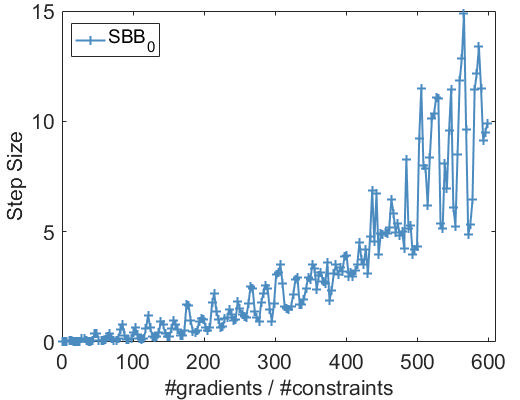
\includegraphics[width = 0.4\columnwidth]{sythetic_tste_0911_sbb_0_cropped.jpg}
		%\caption{the distribution of the nodes in the study site}
		\label{fig:syth:tste:bb:step}
	}
	\subfloat[{SBB$_{0.005}$ step size}]
	{
		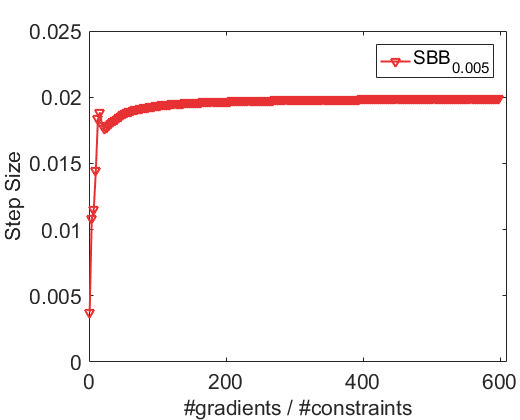
\includegraphics[width = 0.4\columnwidth]{sythetic_tste_1110_sbb_005_step_cropped.jpg}
		%\caption{the distribution of the nodes in the study site}
		\label{fig:syth:tste:rbb:step}
	}
	\caption{Step sizes along iterations of SVRG-SBB$_\epsilon$ on the synthetic data. (a) SBB step size with $\epsilon=0$, (b) SBB step size with $\epsilon=0.005$.}
	\label{fig:step}
\end{figure}
%
%\textit{ Figures of BB step size. comments based on the figure}
%
%\commmk{In Figure~\ref{fig:syth:tste:bb:step}, we could observe that the step sizes generated by SVRG-BB for non-convex ordinal embedding function (\ref{eq:student}) on the synthetic data are changed dramatically. The original non-convex SVRG \cite[Theorem 2]{pmlr-v48-reddi16} could archive an approximate stationary point for the finite-sum problem with constant step size in all epochs, but a very huge step size would makes \cite[Theorem 2]{pmlr-v48-reddi16} no longer true and the results of the SVRG-BB would not be stable. The details of this simulated study will be described in the Experiment section \ref{section:experiment}.}

\subsection{B. Stabilized BB step size}

An intuitive way to overcome the flaw of BB step size is to add another positive term in the absolute value of the denominator of the original BB step size, which leads to our introduced stabilized Barzilai-Borwein (SBB) step size shown as follows,
\begin{equation}
	\label{eq:rbb_step}
	\begin{aligned}
		& \eta_{s} &=&\ \ \frac{1}{m}\cdot\left\|\tilde{\mathbf{X}}^{s}-\tilde{\mathbf{X}}^{s-1}\right\|^2_F\\
		& &\times& \ \ \left(\left|\text{vec}(\tilde{\mathbf{X}}^{s}-\tilde{\mathbf{X}}^{s-1})^T\text{vec}(\mathbf{g}^s-\mathbf{g}^{s-1})\right|\right.\\
		& &+&\ \ \left.\epsilon\left\|\tilde{\mathbf{X}}^{s}-\tilde{\mathbf{X}}^{s-1}\right\|^2_F\right)^{-1}, \quad \text{for some} \  \epsilon>0.
	\end{aligned}
\end{equation}
By the use of SBB step size, the SVRG-SBB algorithm is presented in Algorithm \ref{alg:svrg-bb}.

Actually, as shown by our latter theorem (i.e., Theorem \ref{svrg_bb_nonconvex}), if the Hessian of the objective function $\nabla^2 F(X)$ is nonsingular and the magnitudes of its eigenvalues are lower bounded by some positive constant $\mu$, then we can take $\epsilon=0$. In this case, we call the referred step size SBB$_0$ henceforth. Even if we have no information of the Hessian of the objective function in practice, the SBB$_\epsilon$ step size with an $\epsilon>0$ is just a more consecutive step size of SBB$_0$ step size.



From \eqref{eq:rbb_step}, if the gradient $\nabla F$ is Lipschitz continuous with constant $L>0$, then the SBB$_\epsilon$ step size can be bounded as follows
\begin{align}
\label{eq:bound-rbb}
\frac{1}{m(L+\epsilon)} \leq \eta_k \leq \frac{1}{m\epsilon},
\end{align}
where the lower bound is obtained by the $L$-Lipschitz continuity of $\nabla F$, and the upper bound is directly derived by its specific form.
If further $\nabla^2 F(X)$ is nonsingular and the magnitudes of its eigenvalues has a lower bound $\mu>0$,
then the bound of SBB$_0$ becomes
\begin{align}
\label{eq:bound-rbb0}
\frac{1}{m L} \leq \eta_k \leq \frac{1}{m \mu}.
\end{align}

As shown in Figure \ref{fig:step} (b), SBB$_\epsilon$ step size with a positive $\epsilon$ can make SBB$_0$ step size more stable when SBB$_0$ step size is unstable and varies dramatically. Moreover, SBB$_\epsilon$ step size usually changes significantly only at the initial several epoches, and then quickly gets very stable. This is mainly because there are many iterations in an epoch of SVRG-SBB, and thus, the algorithm might close to a stationary point after only one epoch, and starting from the second epoch, the SBB$_\epsilon$ step sizes might be very close to the inverse of the sum of the curvature of objective function and the parameter $\epsilon$ used.

%The RBB step size (\ref{eq:rbb_step}) is clearly positive. Moreover, (\ref{eq:rbb_step}) is more conservative and practical when the BB step size (\ref{eq:bb_step}) tends to infinity.
%\textit{ give comments on the behavior of RBB based on the figure, and algorithm is presented here}
%\commmk{In Figure~\ref{fig:syth:tste:rbb:step}, the RBB step sizes obtained by (\ref{eq:rbb_step}) under the same setting of BB step sizes are much smaller. We notice that the RBB step size looks like the fixed step size. It would happen when the $\text{vec}(\tilde{\mathbf{X}}^{s}-\tilde{\mathbf{X}}^{s-1})^T\text{vec}(\mathbf{g}^s-\mathbf{g}^{s-1})$ trends to $0$ and $\epsilon\|\tilde{\mathbf{X}}^{s}-\tilde{\mathbf{X}}^{s-1}\|^2_F$ would dominate the denominator. The RBB step size (\ref{eq:rbb_step}) would trends to be $\frac{1}{m\epsilon}$ which is the upper bound of $\{\eta_{s+1}\}$.}


%\begin{algorithm}
%	\small
%	\caption{SVRG-SBB for \eqref{eq:2}}\label{alg:svrg-bb}
%	\begin{algorithmic}
%		\REQUIRE
%        $\scriptstyle\epsilon\geq0$, update frequency $m$, maximal number of iterations $S$, initial step size $\scriptstyle\eta_0$ (only used in the first epoch), initial point $\scriptstyle\tilde{\bf X}^0 \in \mathbb{R}^{n\times d}$, and $\scriptstyle N: = |{\cal P}|$
%		\FOR{$\scriptstyle s=0$ to $\scriptstyle S-1$}
%		\STATE $\scriptstyle \mathbf{g}^{s} = \nabla F(\tilde{\mathbf{X}}^s) =\frac{1}{N}\sum^N_{i=1}\nabla f_i(\tilde{\mathbf{X}}^s)$
%%		\IF {$s>0$ and use BB step size}
%%		\STATE
%%		\begin{equation}
%%			%			\tag{\ref{eq:bb_step}}
%%			\eta_{s+1} = \frac{1}{m}\frac{\|\tilde{\mathbf{X}}^{s}-\tilde{\mathbf{X}}^{s-1}\|^2_F}{\text{vec}(\tilde{\mathbf{X}}^{s}-\tilde{\mathbf{X}}^{s-1})^T\text{vec}(\mathbf{g}_s-\mathbf{g}_{s-1})}
%%		\end{equation}
%%		\ENDIF
%		\IF {$\scriptstyle s>0$}
%		\STATE
%		\begin{equation}
%			\scriptstyle
%			\tag{\ref{eq:rbb_step}}
%			\eta_{s} = \frac{1}{m}\cdot\frac{\|\tilde{\mathbf{X}}^{s}-\tilde{\mathbf{X}}^{s-1}\|^2_F}{|\text{vec}(\tilde{\mathbf{X}}^{s}-\tilde{\mathbf{X}}^{s-1})^T\text{vec}(\mathbf{g}_s-\mathbf{g}_{s-1})|+\epsilon\|\tilde{\mathbf{X}}^{s}-\tilde{\mathbf{X}}^{s-1}\|^2_F}
%		\end{equation}
%		\ENDIF
%		%\STATE $\scriptstyle\eta_{s+1} = \eta_0$
%        \STATE $\scriptstyle\mathbf{X}^{s}_0=\tilde{\mathbf{X}}^s$		
%		\FOR{$ \scriptstyle t=0$ to $\scriptstyle m-1$}
%		\STATE uniformly randomly pick $\scriptstyle i_t\in \{1,\ldots,N\}$
%		\STATE $\scriptstyle\mathbf{X}^{s}_{t+1}= \mathbf{X}^{s}_{t}-\eta_{s}(\nabla f_{i_t}(\mathbf{X}^{s}_{t})-\nabla f_{i_t}(\tilde{\mathbf{X}}^s)+\mathbf{g}^{s})$
%		\ENDFOR
%		\STATE $\scriptstyle \tilde{\mathbf{X}}^{s+1}=\mathbf{X}^{s}_{m}$
%		\ENDFOR
%		\ENSURE ${\scriptstyle \mathbf{X}_{\mathrm{out}}}$ is chosen uniformly from $\scriptstyle\{\{\mathbf{X}^{s}_{t}\}_{t=1}^{m}\}_{s=1}^{S}$.
%	\end{algorithmic}
%\end{algorithm}

\begin{algorithm}[ht]
	\caption{SVRG-SBB for \eqref{eq:2}}
	\label{alg:svrg-bb}
	\KwIn{$\scriptstyle\epsilon\geq0$, update frequency $m$, maximal number of iterations $S$, initial step size $\scriptstyle\eta_0$ (only used in the first epoch), initial point $\scriptstyle\tilde{\bf X}^0 \in \mathbb{R}^{n\times d}$, and $\scriptstyle N: = |{\cal P}|$}
	\KwOut{${\scriptstyle \mathbf{X}_{\mathrm{out}}}$ is chosen uniformly from $\scriptstyle\{\{\mathbf{X}^{s}_{t}\}_{t=1}^{m}\}_{s=1}^{S}$}
	\For{$\scriptstyle s=0$ to $\scriptstyle S-1$}
	{
		$\scriptstyle \mathbf{g}^{s} = \nabla F(\tilde{\mathbf{X}}^s) =\frac{1}{N}\sum^N_{i=1}\nabla f_i(\tilde{\mathbf{X}}^s)$\;
		\If{$\scriptstyle s>0$}
		{
			\begin{equation}
				\scriptstyle
				\tag{\ref{eq:rbb_step}}
				\eta_{s} = \frac{1}{m}\cdot\frac{\|\tilde{\mathbf{X}}^{s}-\tilde{\mathbf{X}}^{s-1}\|^2_F}{|\text{vec}(\tilde{\mathbf{X}}^{s}-\tilde{\mathbf{X}}^{s-1})^T\text{vec}(\mathbf{g}_s-\mathbf{g}_{s-1})|+\epsilon\|\tilde{\mathbf{X}}^{s}-\tilde{\mathbf{X}}^{s-1}\|^2_F}\;
			\end{equation}
		}
		$\scriptstyle\mathbf{X}^{s}_0=\tilde{\mathbf{X}}^s$\;
		\For{$ \scriptstyle t=0$ to $\scriptstyle m-1$}
		{
			uniformly randomly pick $\scriptstyle i_t\in \{1,\ldots,N\}$\;
			$\scriptstyle\mathbf{X}^{s}_{t+1}= \mathbf{X}^{s}_{t}-\eta_{s}(\nabla f_{i_t}(\mathbf{X}^{s}_{t})-\nabla f_{i_t}(\tilde{\mathbf{X}}^s)+\mathbf{g}^{s})$\;
		}
		$\scriptstyle \tilde{\mathbf{X}}^{s+1}=\mathbf{X}^{s}_{m}$\;
	}
\end{algorithm}

\subsection{C. Convergence Results}

In this subsection, we establish the convergence rate of SVRG-SBB as shown in the following theorem.
%In Algorithm~\ref{alg:svrg-bb}, we incorporate the SVRG with RBB step size for non-convex objective functions in (\ref{eq:2}) to work out a fully adaptive stochastic algorithm that can compute the step size automatically. The following theorem shows the convergence of Algorithm~\ref{alg:svrg-bb} with RBB step size.

\begin{theorem}
\label{svrg_bb_nonconvex}
Let $\{\{{\bf X}_t^s\}_{t=1}^m\}_{s=1}^S$ be a sequence generated by Algorithm \ref{alg:svrg-bb}.
Suppose that $F$ is smooth, and $\nabla F$ is Lipschitz continuous with Lipschitz constant $L>0$ and bounded. For any $\epsilon>0$, if
\begin{align}
\label{Eq:cond-m}
m > \max \left\{ 2L^2\left(1+\frac{2L}{\epsilon}\right), 1+ \sqrt{1+\frac{8L^2}{\epsilon^2}}\right\} \cdot \epsilon^{-1},
\end{align}
then for the output ${\bf X}_{\mathrm{out}}$ of Algorithm \ref{alg:svrg-bb}, we have
\begin{align}
\label{eq:rate}
\mathbb{E}[\|\nabla F({\bf X}_{\mathrm{out}})\|^2] \leq \frac{F(\tilde{\bf X}^0)-F({\bf X}^*)}{T \cdot \gamma_S},
\end{align}
where ${\bf X}^*$ is an optimal solution of \eqref{eq:2}, $T = m \cdot S$ is the total number of iterations, $\gamma_S$ is some positive constant satisfying
\[
\gamma_S \geq \min_{0\leq s \leq S-1} \left\{ \eta_s \left[ \frac{1}{2} - \eta_s\left(1+4(m-1)L^3\eta_s^2\right)\right]\right\},
\]
and $\{\eta_s\}_{s=0}^{S-1}$ are SBB step sizes specified in \eqref{eq:rbb_step}.

If further the Hessian $\nabla^2 F(X)$ exists and $\mu$ is the lower bound of the magnitudes of eigenvalues of $\nabla^2 F(X)$ for any bounded $X$, then the convergence rate \eqref{eq:rate} still holds for SVRR-SBB  with $\epsilon$ replaced by $\mu+\epsilon$. In addition, if $\mu>0$, then we can take $\epsilon=0$, and \eqref{eq:rate} still holds for SVRR-SBB$_0$ with $\epsilon$ replaced by $\mu$.
\end{theorem}

Theorem \ref{svrg_bb_nonconvex} is an adaptation of \cite[Theorem 2]{pmlr-v48-reddi16} via noting that the used SBB step size specified in \eqref{eq:rbb_step} satisfies \eqref{eq:bound-rbb}.
The proof of this theorem is presented in supplementary material. Theorem~\ref{svrg_bb_nonconvex} shows certain non-asymptotic rate of convergence of the Algorithm~\ref{alg:svrg-bb} in the sense of convergence to a stationary point.
%With sufficient large $m$ (\ref{Eq:cond-m}) and note $T = mS$, the rate of SVRG-RBB is $\mathcal{O}(\frac{1}{T})$.
%To enable a fair comparison with SGD \cite{ghadimi2013stochastic}, we assume that the total number of iterations in SGD is $T$ and the rate of SGD is $\mathcal{O}(\frac{1}{\sqrt{T}})$.
Similar convergence rates of SVRG under different settings have been also shown in \cite{pmlr-v48-reddi16,pmlr-v48-allen-zhua16}.
% , SVRG-RBB has the same rate but it can automatically obtained the step size and assure the convergence. The step size used in SVRG \cite{pmlr-v48-reddi16,pmlr-v48-allen-zhua16} is related to the Lipschitz constant $L$ which is always had to estimate and the appropriate step size need to be tuned empirically.

Note that the Lipschitz differentiability of the objective function is crucial for the establishment of the convergence rate of SVRG-SBB in Theorem \ref{svrg_bb_nonconvex}. In the following, we give a lemma to show that a part of aforementioned objective functions (\ref{eq:scale-invariant}), (\ref{eq:logistic}) and (\ref{eq:student}) in the ordinal embedding problem are Lipschitz differentiable. Considering the limited space of this paper, the readers are refered to (\url{}) for detailed proofs.
%with bounded $\mathbf{X}$, which is absolutely basic to the convergence analysis.
%The full derivation is given in the supplementary material.
	
\begin{lemma}
\label{lemma:1}
The ordinal embedding functions (\ref{eq:scale-invariant}), (\ref{eq:logistic}) and (\ref{eq:student}) are Lipschitz differentiable for any bounded variable $X$.
\end{lemma}

%\textit{ \subsection{D. Discussions}}
%
%%\textbf{Remarks. }There are a few remarks on the SVRG-RBB non-convex ordinal embedding algorithm.
%\begin{enumerate}
%	%\item If we always set $\eta_{s} = \eta_0$ in SVRG-RBB instead of using (\ref{eq:bb_step}) or (\ref{eq:rbb_step}), Algorithm~\ref{alg:svrg-bb} reduces to the SVRG for non-convex ordinal embedding.
%	
%	\item One may notice that the $\eta_{s+1}$ in (\ref{eq:bb_step}) and (\ref{eq:rbb_step}) is different with which used in \cite{NIPS2016_6286}. Here we treat $\tilde{\mathbf{X}}^{s-1}, \tilde{\mathbf{X}}^{s}, \mathbf{Y}_{s-1}$ and $\mathbf{Y}_s$ as $pn\times 1$ vector in our experiment.
%	
%	\item The main difference between Theorem \ref{svrg_bb_nonconvex} and the result of \cite{NIPS2016_6286} is the \cite{NIPS2016_6286} prove that SVRG-BB converges linearly for strongly convex objective functions, but (\ref{eq:2}) is non-convex finite-sum problems. We can't use co-coercivity (Lemma 3.4 in \cite{NIPS2016_6286}) to obtain the upper bound of $\|\nabla f_{p_t}(\mathbf{X}^{s+1}_{t+1})-\nabla f_{p_t}(\mathbf{X}^*)\|^2$ for bounding $\mathbf{E}[\|\tilde{\mathbf{X}}^{s+1}-\mathbf{X}^*\|]$. Moreover, the original BB method (\ref{eq:bb_step}) is not appropriate for non-convex function as we have been discussed. This theorem for RBB step size is the first theoretical result of BB method in stochastic non-convex optimization.
%
%	%	\item As we use the RBB step size $\eta_{s+1}$ computed in Algorithm \ref{alg:svrg-bb} instead of the fixed step size $\eta_0$, the $\beta^{s+1}_t$ and $m$ get the corresponding constraints to keep $\Gamma^{s+1}_t>0$. By this theorem, we obtain an explicit dependence between the convergence and parameters.
%	
%	\item As the Lipschitz constant of $\nabla F$ for ordinal embedding function (\ref{eq:scale-invariant}), (\ref{eq:logistic}), (\ref{eq:student}) is hard to estimate, we choose $\epsilon$  between $[0.01, 0.02]$ in simulated study and $[1 \times 10^{-5}, 2 \times 10^{-5}]$ in real-world data.
%\end{enumerate}

\section{Experiments}
\label{section:experiment}
 In this section, we conduct a series of simulations and real-world data experiments to demonstrate the effectiveness of the proposed algorithms.
 Three models including \textit{GNMDS}, \textit{STE} and \textit{TSTE} are taken into consideration. Our source code could be found on the web\footnote{\url{https://github.com/alphaprime/Stabilized_Stochastic_BB}}.
% two examples are exhibited with both simulated and real-world data to illustrate the validity of the analysis above and applications of the methodology proposed.
% The first example is with simulated data while the latter one exploit real-world dataset. In the whole following, we focus on a special case of quadruplets as $i=l$ and $\{i, j, i, k\}\subset[n]^3$. We have discussed the relationship between the triplets and quadruplets in Lemma \ref{lemma:1}. Triplet and quadruplet are both admissible input formats and we follow the same input format as GNMDS/STE/TSTE source codes for the ease of comparisons.
%In all the experiments, $(i, j, k)$ is adopt to indicate the ordinal constraint $d^2_{ij}(\mathbf{X})\leq d^2_{ik}(\mathbf{X})$.
	
\subsection{A. Simulations}

{
	%\renewcommand\baselinestretch{1}
	%\renewcommand\arraystretch{0.8}
	\begin{table}[tbh!]
		\centering
		\caption{Computational complexity (second) comparisons on the synthetic dataset.}
		\resizebox{0.9\columnwidth}{!}
		{
			\begin{tabular}{c||cccc}
				\hline
				\multicolumn{5}{c}{GNMDS} \\ \hline\hline
				                      & min     & mean   & max    & std     \\ \hline
				  cvx              & 1.6140  & 1.7881 & 1.9390 & 0.0844  \\ \hline
				  ncvx Batch    & 4.5070  & 4.9372 & 5.2910 & 0.1857  \\ \hline
				  ncvx SGD      & 5.3070  & 5.5882 & 5.8970 & 0.1216  \\ \hline
				  ncvx SVRG     & 2.3020  & 2.8919 & 3.5280 & 0.2911  \\ \hline
				  ncvx SVRG-SBB$_0$  & \textbf{0.3500}  & \textbf{0.4347} & \textbf{0.5340} & \textbf{0.0367}  \\ \hline
				  ncvx SVRG-SBB$_\epsilon$ & \textit{0.3570}  & \textit{0.4858} & \textit{0.6070} & \textit{0.0621}  \\
				\hline
				%\multicolumn{5}{c}{CKL} \\ \hline\hline
				%	  & min 	& mean   & max    & std    \\ \hline
				%SGD   & 1.2700  & 1.5374 & 2.0360 & 0.1976 \\ \hline
				%SVRG  & 2.4160  & 2.7475 & 3.3280 & 0.2523 \\ \hline
				%Batch & 3.1130  & 3.5688 & 5.2410 & 0.4694 \\
				%\hline
				\multicolumn{5}{c}{STE} \\ \hline\hline
				                    & min     & mean   & max    & std     \\ \hline
				cvx             & 3.6740  & 3.9442 & 4.1870 & 0.1709  \\ \hline
				ncvx Batch    & 2.4610  & 2.6326 & 2.9110 & 0.1162  \\ \hline
				ncvx SGD      & 1.5000  & 2.1312 & 2.7190 & 0.2740  \\ \hline
				ncvx SVRG     & 1.9930  & 2.4068 & 2.8350 & 0.1935  \\ \hline
				ncvx SVRG-SBB$_0$  & \textit{0.5000}  & \textit{0.6052} & \textit{0.6980} & \textit{0.0660}  \\ \hline
				ncvx SVRG-SBB$_\epsilon$ & \textbf{0.4510}  & \textbf{0.5773} & \textbf{0.6780} & \textbf{0.0515} \\
				\hline
				\multicolumn{5}{c}{TSTE} \\ \hline\hline
				                    & min     & mean   & max     & std    \\ \hline
				ncvx Batch    & 3.9380  & 4.1815 & 4.4790  & 0.1146 \\ \hline
				ncvx SGD      & 6.0410  & 8.2870 & 9.4770  & 0.6863 \\ \hline
				ncvx SVRG     & 1.6090  & 1.9250 & 2.3470  & 0.1807 \\ \hline
				ncvx SVRG-SBB$_0$  & \textit{0.4580}  & \textit{0.7906} & \textit{1.2480}  & \textit{0.1969} \\ \hline
				ncvx SVRG-SBB$_\epsilon$ & \textbf{0.3800}  & \textbf{0.4726} & \textbf{0.5470}  & \textbf{0.0420} \\
				\hline
			\end{tabular}
		}
		\label{tabl:1}
	\end{table}
}

\begin{figure*}[thb!]
	\centering
	\subfloat[GNMDS]
	{
		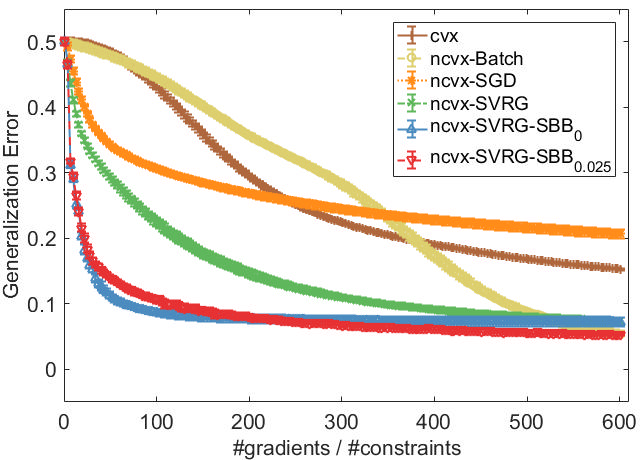
\includegraphics[width = 0.3\textwidth]{sythetic_gnmds_0911_test_cropped.jpg}
		%\caption{the distribution of the nodes in the study site}
		\label{fig:syth:gnmds:error}
	}
	\subfloat[STE]
	{
		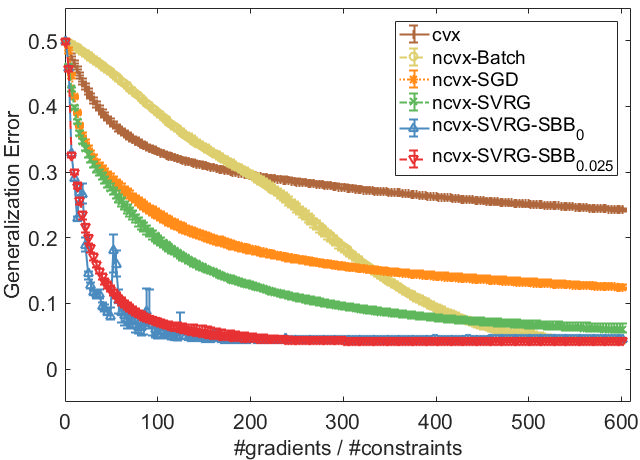
\includegraphics[width = 0.3\textwidth]{sythetic_ste_0911_test_cropped.jpg}
		%\caption{the distribution of the nodes in the study site}
		\label{fig:syth:ste:error}
	}
	\subfloat[TSTE]
	{
		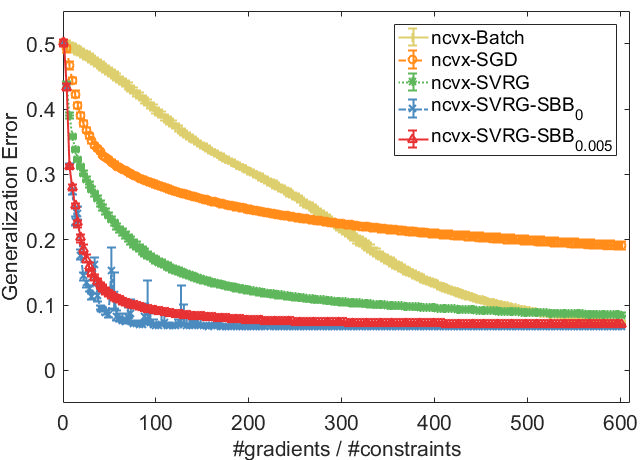
\includegraphics[width = 0.3\textwidth]{sythetic_tste_0911_test_cropped.jpg}
		%\caption{the distribution of the nodes in the study site}
		\label{fig:syth:tste:error}
	}
	\caption{Generalization errors of SGD, SVRG,  SVRG-SBB and batch methods on the synthetic dataset.}
	\label{fig:synthetic}
\end{figure*}

We start with a small-scale synthetic experiment to show how the methods perform in an idealized setting, which provides sufficient ordinal information in noiseless case.
\\\\
\textbf{Settings.} The synthesized dataset consists of $100$ points $\{\mathbf{x}_i\}_{i=1}^{100}\subset\mathbb{R}^{10}$, where $\mathbf{x}_i\sim\mathcal{N}(\mathbf{0}, \frac{1}{20}\mathbf{I})$, where $\mathbf{I}\in \mathbb{R}^{10\times 10}$ is the identity matrix. The possible similarity triple comparisons are generated based on the Euclidean distances between $\{\mathbf{x}_i\}$. As \cite{NIPS2016_6554} has proved that the Gram matrix $\mathbf{G}$ can be recovered from $\mathcal{O}(pn\log n)$ triplets, we randomly choose $|\mathcal{P}|=10,000$ triplets as the training set and the rest as test set. The regularization parameter and step size settings for the convex formulation follow the default setting of the STE/TSTE implementation\footnote{\url{http://homepage.tudelft.nl/19j49/ste/Stochastic_Triplet_Embedding.html}}, so we do not choose the step size by line search or the halving heuristic for convex formulation. The embedding dimension is selected just to be equal to $10$ without variations, because the results of different embedding dimensions have been discussed in the original papers of GNMDS, STE and TSTE.
\\\\
\textbf{Evaluation Metrics. }The metrics that we used in the evaluation of various algorithms include the generalization error and running time. As the learned embedding $\mathbf{X}$ from partial triple comparisons set $\mathcal{P}\subset[n]^3$ may be generalized to unknown triplets, the percentage of held-out triplets which is satisfied in the embedding $\mathbf{X}$ is used as the main metric for evaluating the quality. The running time is the duration of a algorithm when the training error is larger than $0.15$.
\\\\
\textbf{Competitors.} We evaluate both convex and non-convex formulations of three objective functions (i.e. GNMDS, STE and TSTE). We set the two baselines as : ($1$) the convex objective function whose results are denoted as ``convex'', and ($2$) these non-convex objective functions solved by batch gradient descent denoted as ``ncvx batch''. We compare the performance of SVRG-SBB$_\epsilon$ with SGD, SVRG with a fixed step size (called SVRG for short henceforth) as well as the batch gradient descent methods.
%to the convex and non-convex results obtained by batch gradient descent.
As SVRG and its variant (SVRG-SBB$_\epsilon$) runs $2m+|\mathcal{P}|$ times of (sub)gradient in each epoch, the batch and SGD solutions are evaluated with the same numbers of (sub)gradient of SVRG. In Figure~\ref{fig:synthetic}, the $x$-axis is the computational cost measured by the number of gradient evaluations divided by the total number of triple-wise constraints $|\mathcal{P}|$. The generalization error is the result of $50$ trials with different initial $\mathbf{X}_0$. For each epoch, the median number of generalization error over 50 trials with [0.25, 0.75] confidence interval are plotted. The experiment results are shown in Figure \ref{fig:synthetic} and Table \ref{tabl:1}.
% in the figure. %The error bar in the all graphs represents the range between one unit of standard deviation.
%In Figure~\ref{fig:step}, the $x$-axis is the same as Figure~\ref{fig:synthetic} and the $y$-axis is the step size obtained by BB and RBB method.
\\\\
\textbf{Results.}
%Figure \ref{fig:synthetic} shows the experiment results of three objective functions as GNMDS, STE and TSTE.
%From these experimental results, we make the following comments.
From to Figure \ref{fig:synthetic}, the following phenomena can be observed.
First, the algorithm SVRG-SBB$_0$ will be unstable at the initial several epoches for three models, and latter get very stable. The eventual performance of SVRG-SBB$_0$ and that of SVRG-SBB$_\epsilon$ are almost the same in three cases.
Second, compared to the batch methods, all the stochastic methods including SGD, SVRG and SVRG-SBB$_{\epsilon}$ ($\epsilon =0$ or $\epsilon>0$) converge fast at the initial several epoches and quickly get admissible results with relatively small generalization error. This is one of our main motivations to use the stochastic methods. Particularly, for all three models, SVRG-SBB$_\epsilon$ outperforms all the other methods in the sense that it not only converges fastest but also achieves almost the best generalization error. Moreover, the outperformance of SVRG-SBB$_\epsilon$ in terms of the cpu time can be also observed from Table \ref{tabl:1}. Specifically, the speedup of SVRG-SBB$_\epsilon$ over SVRG is about 4 times for all three models.


%it can be seen from this figure that with the increase of gradient computations, the generalization error curve generally decreases. Moreover, we note that at the initial stage, both SGD, SVRG and BB methods could outperform the batch optimization for convex and non-convex formulations with smaller generalization error.

%Furthermore, it can be seen that the SVRG and (R)BB methods are able to maintain competitive performances with the batch case in the long run because of its ``variance-reduction" property.
%
%Figure~\ref{fig:synthetic} displays the different performance of BB step size and RBB step size. The restriction and regularization gives the RBB a huge advantage over BB as RBB is more conservative than BB when $\mathbf{g}_s$ is very close to $\mathbf{g}_{s-1}$. If the step size is exaggerate, the generalization error will increase and the algorithm needs more epoch to archive a stable result. The RBB method uses a feasible step size in the most of the whole procedure and outperform SVRG with fixed step size and BB step size when the three variants of SVRG use the same initial choice of the step size.


Table \ref{tabl:1} shows the computational complexity achieved by SGD, SVRR-SBB$_\epsilon$ and batch gradient descent for convex and non-convex objective functions. All computation is done using MATLAB$^\text{\textregistered{}}$ R2016b, on a desktop PC with Windows$^\text{\textregistered{}}$ $7$ SP$1$ $64$ bit, with $3.3$ GHz Intel$^\text{\textregistered{}}$ Xeon$^\text{\textregistered{}}$ E3-1226 v3 CPU, and $32$ GB $1600$ MHz DDR3 memory. It is easy to see that for all objective functions, SVRG-SBB$_\epsilon$ gains speed-up compared to the other methods. Besides, we notice that the convex methods could be effective when $n$ is small as the projection operator will not be the bottleneck of the convex algorithm.
%Finally, we stress that (R)BB make use of the gradient computation more efficiently than batch, SGD and SVRG method.
%\\\\
%{
%	\renewcommand\baselinestretch{1}
%	\renewcommand\arraystretch{1.0}
%	\begin{table}[tbh]
%		\centering
%		\small
%		\caption{Computational complexity (second.) comparison on the music artist dataset.}
%		\resizebox{0.97\columnwidth}{!}
%		{
%			\begin{tabular}{c||cccc}
%				\hline
%				\multicolumn{5}{c}{GNMDS} \\ \hline\hline
%				& min 	  & mean   & max    & std    \\ \hline
%				Convex              & 21.530  & 28.236 & 38.348 & 3.5000 \\ \hline
%				Non-Convex Batch    & 2.7930  & 2.9874 & 3.1720 & \textbf{0.0917} \\ \hline
%				Non-Convex SGD      & -       & -      & -      & -      \\ \hline
%				Non-Convex SVRG     & 4.7750  & 5.3532 & 5.7080 & 0.2579 \\ \hline
%				Non-Convex SVRG-BB  & \textbf{1.3380}  & \textbf{1.8902} & \textbf{2.4530} & 0.3550 \\
%				\hline
%				%\multicolumn{5}{c}{CKL} \\ \hline\hline
%				%	  & min 	& mean   & max    & std    \\ \hline
%				%SGD   & 0.2990  & 0.3733 & 0.4690 & 0.0397 \\ \hline
%				%SVRG  & 1.3130  & 1.5706 & 1.8490 & 0.1049 \\ \hline
%				%Batch & 1.3540  & 1.7107 & 3.1700 & 0.4112 \\
%				%\hline
%				\multicolumn{5}{c}{STE} \\ \hline\hline
%				& min     & mean   & max    & std     \\ \hline
%				Convex              & -       & -      & -      & -       \\ \hline
%				Non-Convex Batch    & 2.9060  & 3.0713 & 3.7880 & \textbf{0.2122}  \\ \hline
%				Non-Convex SGD      & -       & -      & -      & -       \\ \hline
%				Non-Convex SVRG     & 8.9850  & 10.086 & 11.366 & 0.4867  \\ \hline
%				Non-Convex SVRG-BB  & \textbf{1.3700}  & \textbf{2.5650} & \textbf{3.4080} & 0.4929  \\
%				
%				\hline
%				\multicolumn{5}{c}{TSTE} \\ \hline\hline
%				& min     & mean   & max     & std    \\ \hline
%				Batch    & -       & -      & -       & -      \\ \hline
%				SGD      & -       & -      & -       & -      \\ \hline
%				SVRG     & 2.2670  & 2.4591 & 2.8350  & 0.6545 \\ \hline
%				SVRG-BB  & \textbf{0.4230}  & \textbf{0.4771} & \textbf{0.7150}  & \textbf{0.0848} \\ \hline
%				
%			\end{tabular}
%		}
%		\label{tabl:2}
%	\end{table}
%}
{
	%\renewcommand\baselinestretch{1}
	%\renewcommand\arraystretch{0.8}
	\begin{table*}[tbh]
		%\small
		\centering
		\caption{Image retrieval performance (MAP and Precision@40) on SUN397 when $p=19$.}
		%\resizebox{0.9\textwidth}{!}
		{
			\begin{tabular}{c||cc||cc||cc}
				\hline
				& \multicolumn{2}{c||}{$0\%$} & \multicolumn{2}{c||}{$5\%$} & \multicolumn{2}{c}{$10\%$}\\
				&  MAP& Precision@40 & MAP 	& Precision@40 & MAP & Precision@40 \\ \hline\hline
				\multicolumn{7}{c}{GNMDS} \\\hline\hline
				cvx              & 0.2691  & 0.3840  & 0.2512  & 0.3686   & 0.2701  & 0.3883  \\ \hline
				ncvx Batch    & 0.3357  & 0.4492  & 0.3791  & 0.4914   & 0.3835  & 0.4925  \\ \hline
				ncvx SGD      & 0.3245  & 0.4379  & 0.3635  & 0.4772   & 0.3819  & 0.4931  \\ \hline
				ncvx SVRG     & 0.3348  & 0.4490  & \textit{0.3872}  & \textit{0.4974}   & \textit{0.3870}  & \textit{0.4965}  \\ \hline
				ncvx SVRG-SBB$_0$  & \textbf{0.3941}  & \textbf{0.5040}  & 0.3700  & 0.4836   & 0.3550  & 0.4689  \\ \hline
				ncvx SVRG-SBB$_\epsilon$ & \textit{0.3363}  & \textit{0.4500}  & \textbf{0.3887}  & \textbf{0.4981}   & \textbf{0.3873}  & \textbf{0.4987} \\
				\hline\hline
				\multicolumn{7}{c}{STE} \\\hline\hline
				cvx              & 0.2114  & 0.3275  & 0.1776 & 0.2889 & 0.1989 & 0.3190  \\ \hline
				ncvx Batch    & 0.2340  & 0.3525  & 0.2252 & 0.3380 & 0.2297 & 0.3423  \\ \hline
				ncvx SGD      & 0.3369  & 0.4491  & 0.2951 & 0.4125 & 0.2390 & 0.3488  \\ \hline
				ncvx SVRG     & 0.3817  & 0.4927  & 0.3654 & 0.4804 & 0.3245 & 0.4395  \\ \hline
				ncvx SVRG-SBB$_0$  & \textbf{0.3968}   & \textbf{0.5059} & \textbf{0.3958} & \textbf{0.5054} & \textit{0.3895} & \textbf{0.5002}  \\ \hline
				ncvx SVRG-SBB$_\epsilon$ & \textit{0.3940}  & \textit{0.5036}  & \textit{0.3921} & \textit{0.5012} & \textbf{0.3896} & \textit{0.4992}  \\
				\hline\hline
				\multicolumn{7}{c}{TSTE} \\\hline\hline
				ncvx Batch    & 0.2268  & 0.3470  & 0.2069  & 0.3201 & 0.2275  & 0.3447  \\ \hline
				ncvx SGD      & 0.2602  & 0.3778  & 0.2279  & 0.3415 & 0.2402  & 0.3514  \\ \hline
				ncvx SVRG     & 0.3481  & 0.4617  & 0.3160  & 0.4332 & 0.2493  & 0.3656  \\ \hline
				SVRG-SBB$_0$             &\textbf{0.3900}    & \textbf{0.4980}  & \textbf{0.3917}  & \textbf{0.5018} & \textbf{0.3914}  & \textit{0.5007}  \\ \hline
				ncvx SVRG-SBB$_\epsilon$ & \textit{0.3625}  & \textit{0.4719}  & \textit{0.3845}  & \textit{0.4936} & \textit{0.3897}  & \textbf{0.5013} \\
				\hline\hline
			\end{tabular}
		}
		\label{tabl:3}
	\end{table*}
}

\begin{figure*}[thb!]
	\centering
	\subfloat[GNMDS]
	{
		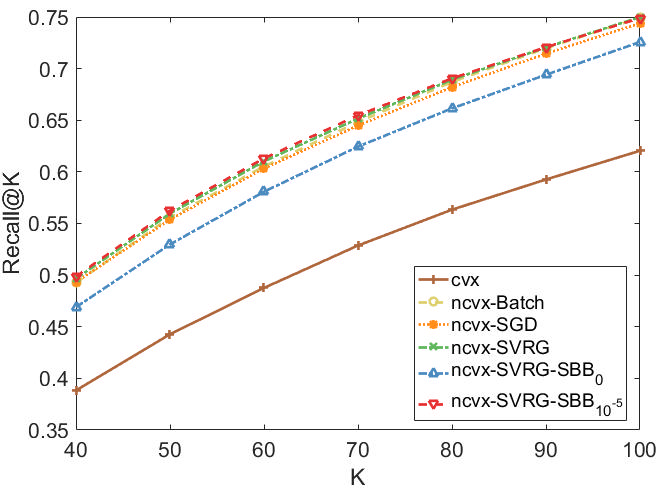
\includegraphics[width=0.3\textwidth]{sun_gnmds_0917_10_cropped.jpg}
		%\caption{the distribution of the nodes in the study site}
		\label{fig:imagenet:gnmds}
	}
	\subfloat[STE]
	{
		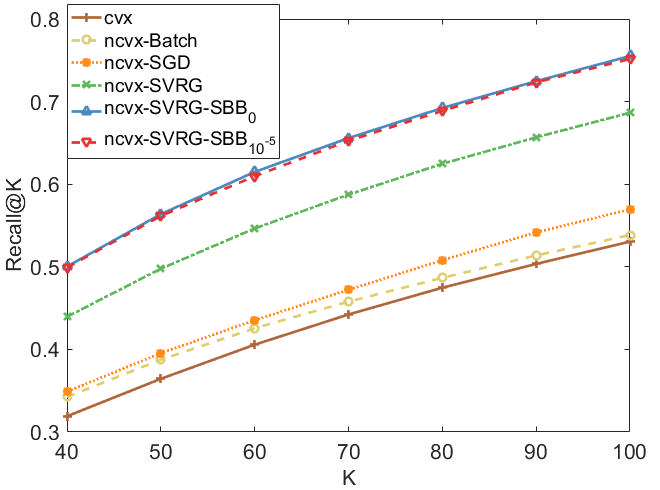
\includegraphics[width=0.3\textwidth]{sun_ste_0917_10_cropped.jpg}
		%\caption{the distribution of the nodes in the study site}
		\label{fig:imagenet:ste}
	}
	\subfloat[TSTE]
	{
		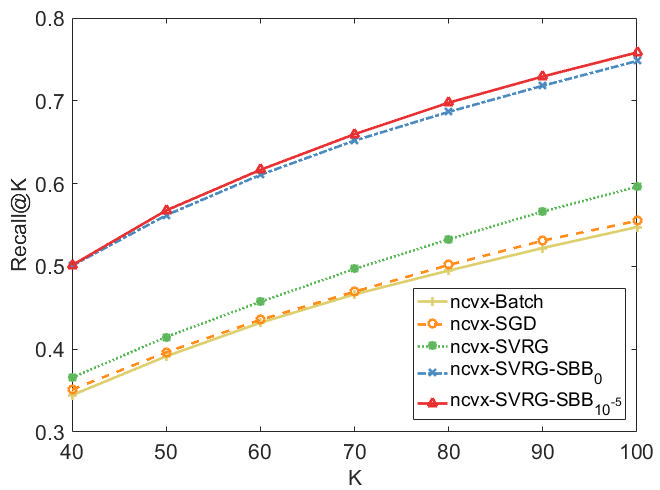
\includegraphics[width=0.3\textwidth]{sun_tste_0917_10_cropped.jpg}
		%\caption{the distribution of the nodes in the study site}
		\label{fig:imagenet:tste}
	}
	%\subfigure[CKL]
	%{
	%	\includegraphics[scale = 0.25]{final_sythetic_gnmds_five_method_20170212.png}
	%	%\caption{the distribution of the nodes in the study site}
	%	\label{fig:syth:ckl}
	%}
	\caption{Recall@K with $10\%$ noise on SUN397.}
	\label{fig:sun} %% label for entire figure
\end{figure*}

%\textbf{Remark. }Step size is a critical parameter in gradient method and we adopt different strategies for the three optimization methods in experiments. The step size of batch gradient descent is adjusted with an adaptive mechanism as: when objective function value $f(\mathbf{X}_t)$ is larger than $f(\mathbf{X}_{t-1})$, the step size is $\eta_t=1.01\eta_{t-1}$; when $f(\mathbf{X}_t)$ is smaller than $f(\mathbf{X}_{t-1})$, the step size is $\eta_t=0.5\eta_{t-1}$. We decrease the step size $\eta_t$ of SGD by step size scheduling as: exponential decay $\eta_t = \eta_0 a^{\left \lfloor \frac{t}{|\mathcal{P}|} \right \rfloor}$ with parameters $\eta_0$ and $a$ to adjust. For SVRG, we utilize a fixed step size. The relatively large $\eta$ with SVRG will lead to faster convergence than that of SGD. The step size of SVRG-BB and SVRG-RR are calculated as (\ref{eq:bb_step}) and (\ref{eq:rbb_step}).
%	
%\begin{figure*}[thb!]
%	\centering
%	\subfloat[GNMDS]
%	{
%		\includegraphics[width=0.31\textwidth]{final_music_gnmds_five_method_20170212-iloveimg-cropped.png}
%		%\caption{the distribution of the nodes in the study site}
%		\label{fig:music:gnmds}
%	}
%	\subfloat[STE]
%	{
%		\includegraphics[width=0.31\textwidth]{final_music_ste_five_method_20170212-iloveimg-cropped.png}
%		%\caption{the distribution of the nodes in the study site}
%		\label{fig:music:ste}
%	}
%	\subfloat[TSTE]
%	{
%		\includegraphics[width=0.31\textwidth]{final_music_tste_four_method_20170212-iloveimg-cropped.png}
%		%\caption{the distribution of the nodes in the study site}
%		\label{fig:music:tste}
%	}
%	\caption{Generalization error of SGD, SVRG(-BB) and batch optimization on the music artist dataset.}
%	\label{fig:3} %% label for entire figure
%\end{figure*}
	
% \subsection{Music Artist Data}
% 	
%  In this experiment, we evaluate how the convex and non-convex ordinal embedding methods perform in a real-world setting with insufficient ordinal constraints.
% 	
% \textbf{Settings. }The music artist data is collected by \cite{ellis2002quest} via a web-based survey in which $1,032$ users provided $213,472$ triplets on the similarity of $412$ music artists. We use the data pre-processed by \cite{vandermaaten2012stochastic} which includes only $9,107$ triplets for $n=400$ artists. For each trial of the dataset, $80\%$ triplets are randomly picked as the training set and the rest as the testing set. The desired dimension of embedding is $p=9$ as these music artists can be classified by genre into $9$ categories.
% 	
% \textbf{Results. }From Figure \ref{fig:3} and Table \ref{tabl:2}, we have the following observations. First, the generalization error gap of convex and non-convex methods are small in this dataset. We speculate that it is due to the training set of this experiment only provide little ordinal information. Second, the batch method is efficient in this small-scale dataset as the calculation of the full gradient is not expensive in this case. Third, the SVRG-RBB method is often significantly faster than the other method as it benefits from the variable step sizes in each epoch. In a word, even with insufficient triple-wise comparisons, the SVRG-BB, could reach comparable accuracy to batch learning, yet with faster speeds.

\subsection{B. Image Retrieval on SUN397}

%Our primary motivation for the development of ordinal embedding algorithm is the analysis of how relative comparisons perceive the similarities of data objects.
Here, we apply the proposed SVRG-SBB algorithm for a real-world dataset, i.e., SUN 397, which is generally used for the image retrieval task.
In this experiment, we wish to see how the learned representation characterizes the ``relevance'' of the same image category and the ``discrimination'' of different image categories. Hence, we use the image representation obtained by ordinal embedding for image retrieval.
\\\\
\textbf{Settings. }We evaluate the effectiveness of the proposed stochastic non-convex ordinal embedding method for visual search on the SUN397 dataset. SUN$397$ consists of around 108K images from $397$ scene categories. In SUN$397$, each image is represented by a $1,600$-dimensional feature vector extracted by principle component analysis (PCA) from $12,288$-dimensional Deep Convolution Activation Features \cite{Gong2014}. We form the training set by randomly sampling $1,080$ images from $18$ categories with $60$ images in each category. Only the training set is used for learning an ordinal embedding and a nonlinear mapping from the original feature space to the embedding space whose dimension is $p=18$. The nonlinear mapping is used to predict the embedding of images which do not participate in the relative similarity comparisons. We use Regularized Least Square and Radial basis function kernel to obtain the nonlinear mapping.  The test set consists of $720$ images randomly chose from $18$ categories with $40$ images in each category.  We use ground truth category labels of training images to generate the triple-wise comparisons without any error. The ordinal constraints are generated like \cite{7410580}: if two images $i,\ j$ are from the same category and image $k$ is from the other categories, the similarity between $i$ and $j$ is larger than the similarity between $i$ and $k$, which is indicated by a triplet $(i,j,k)$. The total number of such triplets is $70,000$. Errors are then synthesized to simulate the human error in crowd-sourcing. We randomly sample $5\%$ and $10\%$ triplets to exchange the positions of $j$ and $k$ in each triplet $(i,j,k)$.
\\\\
\textbf{Evaluation Metrics.} To measure the effectiveness of various ordinal embedding methods for visual search, we consider three evaluation metrics, \textit{i.e.}, precision at top-K positions (Precision@K), recall at top-K positions (Recall@K), and Mean Average Precision (MAP). Given the mapping feature $\mathbf{X}=\{\mathbf{x}_1, \mathbf{x}_2,\dots,\mathbf{x}_{720}\}$ of test images and chosen an image $i$ belonging to class $c_i$ as a query, we sort the other images according to the distances between their embeddings and $\mathbf{x}_i$ in an ascending order as $\mathcal{R}_i$. True positives ($\text{TP}^K_i$) are images correctly labeled as positives, which involve the images belonging to $c_i$ and list within the top K in $\mathcal{R}_i$. False positives ($\text{FP}^K_i$) refer to negative examples incorrectly labeled as positives, which are the images belonging to $c_l(l\neq i)$ and list within the top K in $\mathcal{R}_i$. True negatives ($\text{TN}^K_i$) correspond to negatives correctly labeled as negatives, which refer to the images belonging to $c_l(l\neq i)$ and list after the top K in $\mathcal{R}_i$. Finally, false negatives ($\text{FN}^K_i$) refer to positive examples incorrectly labeled as negatives, which are relevant to the images belonging to class $c_i$ and list after the top K in $\mathcal{R}_i$. We are able to define Precision@K and Recall@K used in this paper as:
$
	\text{Precision@}K = \frac{1}{n}\sum_i^{n}p_i^K=\frac{1}{n}\sum_i^{n}\frac{\text{TP}^K_i}{\text{TP}^K_i+\text{FP}^K_i}
$
and
$
	\text{Recall@}K = \frac{1}{n}\sum_i^{n}r_i^K=\frac{1}{n}\sum_i^{n}\frac{\text{TP}^K_i}{\text{TP}^K_i+\text{FN}^K_i}.
$
Precision and recall are single-valued metrics based on the whole ranking list of images determined by the Euclidean distances among the embedding $\{\mathbf{x}_i\}_{i=1}^n$. It is desirable to also consider the order in which the images from the same category are embedded. By computing precision and recall at every position in the ranked sequence of the images for query $i$, one can plot a precision-recall curve, plotting precision $p_i(r)$ as a function of recall $r_i$. Average Precision(AP) computes the average value of $p_i(r)$ over the interval from $r_i=0$ to $r_i=1$: $\text{AP}_i = \int_{0}^1 p_i(r_i)dr_i$, which is the area under precision-recall curve. This integral can be replaced with a finite sum over every position $q$ in the ranked sequence of the embedding: $\text{AP}_i = \sum_{q=1}^{40} p_i(q)\cdot\triangle r_i(q)$, where $\triangle r_i(q)$ is the change in recall from items $q-1$ to $q$. The MAP used in this paper is defined as $\text{MAP} = \frac{1}{n}\sum_{i=1}^{n}\text{AP}_i$.
\\\\
\textbf{Results.} The experiment results are shown in Table \ref{tabl:3} and Figure \ref{fig:sun}.
As shown in Table \ref{tabl:3} and Figure \ref{fig:sun} with $K$ varying from $40$ to $100$, we observe that non-convex SVRG-SBB$_\epsilon$ consistently achieves the superior Precision@K, Recall@K and MAP results comparing against the other methods with the same gradient calculation. The results of GNMDS illustrate that SVRG-SBB$_\epsilon$ is more suitable for non-convex objective functions than the other methods. Therefore, SVRG-SBB$_\epsilon$ has a very promising potential in practice, because it generates appropriate step sizes automatically while running the algorithm and the result is robust. Moreover, under our setting and with small noise, all the ordinal embedding methods achieve the reasonable results for image retrieval. It illustrates that high-quality relative similarity comparisons can be used for learning meaningful representation of massive data, thereby making it easier to extract useful information in other applications.

\section{Conclusions}

In this paper, we propose a stochastic non-convex framework for the ordinal embedding problem. We propose a novel stochastic gradient descent algorithm called SVRG-SBB for solving this non-convex framework. The proposed SVRG-SBB is a variant of SVRG method incorporating with the so-called stabilized BB (SBB) step size, a new, stable and adaptive step size introduced in this paper. The main idea of the SBB step size is adding another positive term in the absolute value of the denominator of the original BB step size such that SVRG-SBB can overcome the instability of the original BB step size when applied to such non-convex problem. A series of simulations and real-world data experiments are implemented to demonstrate the effectiveness of the proposed SVRG-SBB for the ordinal embedding problem. It is surprising that the proposed SVRG-SBB outperforms most of the state-of-the-art methods in the perspective of both generalization error and computational cost. We also establish the $O(1/T)$ convergence rate of SVRG-SBB in terms of the convergence to a stationary point. Such convergence rate is comparable to the existing best convergence results of SVRG in literature.

%to learn representation from relative similarity comparisons through stochastic non-convex ordinal embedding.
%By taking advantage of the sparse structure of the gradients, we showed how to operate stochastic optimization algorithm and incorporate RBB to determine a appropriate step size. SGD, SVRG and SVRG-(R)BB were systematically studied. Experimental results on synthetic and real-world datasets show that the proposed SVRG-RBB algorithms can achieve as nearly good performance as the batch counterpart. Moreover, in all cases SVRG-RBB are more robust than SVRG-BB due to the non-convex objective functions are not satisfied the condition of SVRG-BB and the corresponding step size could be exaggerated. For future work, we will improve our ordinal embedding approach by explicitly handling noisy ordinal constraints as they are ubiquitous in real-world applications.% \cite{Xu2016FDRicml}.

\section*{Acknowledgment}
The work of Ke Ma is supported by National Key Research and Development Plan (No.2016YFB0800403), National Natural Science Foundation of China (No.U1605252 and 61733007). The work of Jinshan Zeng is supported in part by the National Natural Science Foundation of China (No.61603162), and the Doctoral start-up foundation of Jiangxi Normal University. The work of Qianqian Xu was supported in part by National Natural Science Foundation of China (No. 61672514), and CCF-Tencent Open Research Fund. Yuan Yao's work is supported in part by Hong Kong Research Grant Council (HKRGC) grant 16303817, National Basic Research Program of China (No. 2015CB85600, 2012CB825501), National Natural Science Foundation of China (No. 61370004, 11421110001), as well as grants from Tencent AI Lab, Si Family Foundation, Baidu BDI, and Microsoft Research-Asia. %The corresponding author of this work is Xiaochun Cao (caoxiaochun@iie.ac.cn) and Yuan Yao (yuany@ust.hk).

\bibliographystyle{aaai}
\bibliography{aaai18}
									
%\subfile{./supple_1125_new.tex}
\end{document}
